% 원본 양식 출처 : http://forcecore.tistory.com/1113
\documentclass{beamer}
% select theme
%\usetheme{Boadilla}%personally, none of the presets suit well in this case
\usecolortheme{lily}

\usepackage[hangul]{kotex}%to input Korean letters
\usepackage{fancyvrb}%fancy verbatim
\usepackage{color}%to use color presets
\usepackage{graphicx}%includegraphics
\usepackage{epstopdf}%enables to include eps by converting to pdf
\usepackage{verbatim}%comment
\usepackage{comment}
\usepackage{gensymb}%\deg
\renewenvironment{comment}{}{}%http://tex.stackexchange.com/questions/45617/comment-package-not-working

%http://tex.stackexchange.com/questions/207261/how-do-i-produce-a-double-flat-symbol-edit
\DeclareFontFamily{U}{musix}{}%
\DeclareFontShape{U}{musix}{m}{n}{%
	<-12>   musix11
	<12-15> musix13
	<15-18> musix16
	<18-23> musix20
	<23->   musix29
}{}%
% Not strictly necessary but convenient:
\newcommand*\musix{\usefont{U}{musix}{m}{n}\selectfont}
\DeclareTextFontCommand{\textmusix}{\musix}
\newcommand*\doubleflat{{\Large\raisebox{.6ex}{\textmusix{3}}}}
\newcommand*\doublesharp{{\Large\raisebox{.6ex}{\textmusix{5}}}}

\setbeamertemplate{navigation symbols}{}%to suppress navigation tools
\setbeamertemplate{footline}[text line]{%
	\parbox{\linewidth}{\vspace*{-8pt}매나니 화성학 강좌\hfill\hfill\insertpagenumber}}%footer

\newcommand{\Rn}[1]{%
	\textup{\uppercase\expandafter{\romannumeral#1}}%
}
\newcommand{\rn}[1]{%
	\textup{\lowercase\expandafter{\romannumeral#1}}%
}
\begin{document}
	
	% title slide
	\begin{frame}
		\title{한 번 해보는 화성학 이야기}
		\author{14080 이상헌}
		\date{}
		\titlepage
	\end{frame}
	
	% outline slide
	%\section*{목차}
	%\begin{frame}
	%	\setcounter{tocdepth}{1}
	%	\tableofcontents
	%\end{frame}

	\section{Section 1 : Preface}\label{sec:preface}%The name of sections are ASCII
	\subsection{First......}
	\begin{frame}
		\frametitle{Section \ref{sec:preface} : 서문}
		\framesubtitle{우선......}
		우선 이 pdf를 보고 있는 당신은, 최소한 음악에 대한 열정이 어느 정도는 있다는 것으로 알겠습니다. 그런 당신에게 우선 큰 박수를 보냅니다.
	\end{frame}
	
	\subsection{A tale of 14080 Sangheon Lee}
	\begin{frame}
		\frametitle{Section \ref{sec:preface} : 서문}
		\framesubtitle{14080 이상헌의 이야기}
		제 이야기부터 조금 해 볼까요?\\
		저는 어릴 때부터 음악을 좋아했습니다. 피아노도 좋아했고, 동네 형들이 당시에는 많았던 오락기들로 리듬게임 구경하는 것도 좋아했어요. 그렇게 든 꿈이 {\bf 작곡을} 하는 것이었습니다. 
	\end{frame}
	
	\begin{frame}
		\frametitle{Section \ref{sec:preface} : 서문}
		\framesubtitle{14080 이상헌의 이야기}
		비단 저만 어릴 때 이런 꿈을 그려왔던 것은 아니겠지요. 그래도 저는 계속 작곡하겠다는 의지를 가졌고, 어쩌다보니 작곡작사동아리 매나니의 부기장이 되어 있었습니다.
	\end{frame}
	
	\begin{frame}
		\frametitle{Section \ref{sec:preface} : 서문}
		\framesubtitle{그런데......}
		그리고 깨달았습니다. {\bf 상대음감}과 {\bf 절대음감}을 동시에 지닌 사람은 생각보다 많지 않다는 걸. 저는 사실 고2 중반때까지만 해도 거의 모든 사람들이 음을 들으면 뭔지 알고 화음 들으면 무슨 화음인지 알 줄 알았어요. 그런데 제가 특이한 인간이더군요......
	\end{frame}
	
	\begin{frame}
		\frametitle{Section \ref{sec:preface} : 서문}
		\framesubtitle{결국 무언가가 필요하다!}
		뭐 사실 화성학을 알고 있는 사람도 이를 이론적으로 알고 있는 경우는 드뭅니다. 음감......으로 커버하는 경우가 대부분이죠. 하지만 기본적인 이론을 보다보면 어느 정도 이해가 되지 않을까라고 생각을 해보았습니다. 그러한 생각에 입각하여 이 설명서를 만들어 나가는 것이고요.
	\end{frame}
	
	\subsection{Warning}
	\begin{frame}
		\frametitle{Section \ref{sec:preface} : 서문}
		\framesubtitle{주의 사항}
		다만 본 pdf를 읽을 때 다음과 같은 주의를 요합니다.
		\begin{itemize}
			\item {\bf 이 자료는 공신력이 없습니다!} 여기 있는 건 어느 정도의 참고자료로만 보세요.
			\item 그리고 저는 화성학을 실속 있게는 가르치겠지만, {\bf 정말 대충 설명할 겁니다. 추가적인 내용은 알아서 검색하세요.}
			\item 이론도 중요하지만, 제일 중요한 건 직접 해보는 겁니다. FL이든 MuseScore든 음을 내보면서 이론을 다잡아보세요.
		\end{itemize}
	\end{frame}
	
	\begin{frame}
		\frametitle{Section \ref{sec:preface} : 서문}
		\framesubtitle{주의 사항}
		\begin{itemize}
			\item 이런 거 다 음감이라고요? 완전히 부인할 수는 없습니다만, {\bf 알고 만드는 거랑 모르고 만드는 거랑은 다릅니다.}
			\item 또, 저는 피아노 이외의 악기를 제대로 배워 본 적이 없기에, 그러한 악기들을 배울 때 자연스럽게 접하는 용어들을 잘 모릅니다. 특히 기타 쪽이요. 감안하고 읽어주시기 바랍니다.
		\end{itemize}
	\end{frame}
	
	\section{Section 2 : What is music?}\label{sec:music}
	\subsection{Definition of music}
	\begin{frame}
		\frametitle{Section \ref{sec:music} : 음악이란?}
		\framesubtitle{음악의 정의}
		\begin{definition}[음악, 音樂, Music]
			\begin{itemize}
				\item 박자, 가락, 음성 따위를 갖가지 형식으로 조화하고 결합하여, 목소리나 악기를 통하여 사상 또는 감정을 나타내는 예술. \\- 표준국어대사전
			\end{itemize}
		\end{definition}
	\end{frame}
	
	\begin{frame}
		\frametitle{Section \ref{sec:music} : 음악이란?}
		\framesubtitle{음악의 정의?}
		......라고 서술은 했습니다만, 사실 음악의 정의는 대단히 어렵습니다. Wikipedia만 해도 `Definition of Music'이라는 문서에서 음악은 주관적인 것이다라는 논조를 펼치고 있고, 그게 사실 맞는 말이기도 합니다. 뭔가 이게 음악이다하는 느낌은 있을 테니까요.
	\end{frame}
	
	\subsection{Elements of sound}
	\begin{frame}
		\frametitle{Section \ref{sec:music} : 음악이란?}
		\framesubtitle{그래도 음악은 소리를 다룬다}
		그럼에도 불구하고 변하지 않는 사실은 음악은 {\bf 소리}를 다룬다는 것입니다. 소리를 구성하는 요소는 4가지 정도가 있습니다.
		\begin{itemize}
			\item \bf 음높이(pitch)
			\item \bf 음정(timbre)
			\item \bf 세기(loudness)
			\item \bf 길이(duration)
		\end{itemize}
	\end{frame}
	
	\begin{frame}
		\frametitle{Section \ref{sec:music} : 음악이란?}
		\framesubtitle{음높이(pitch)}
		주파수에 따라 음의 고저가 나타나게 됩니다. 주파수가 높아질수록 음이 높아지죠. 화성학은 이 진동수에 입각해서 시작되었습니다.
		\begin{columns}
			\begin{column}{0.5\textwidth}
				\centering
				\noindent
				\begin{figure}[h!]
					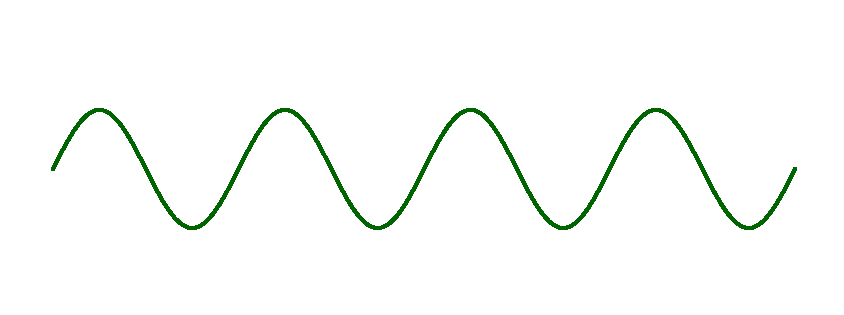
\includegraphics[width=0.9\columnwidth]{res/pdf/2/pitch/A4.eps}
				\end{figure}
				\noindent
			\end{column}
			\begin{column}{0.5\textwidth}
				\centering
				\begin{figure}[h!]
					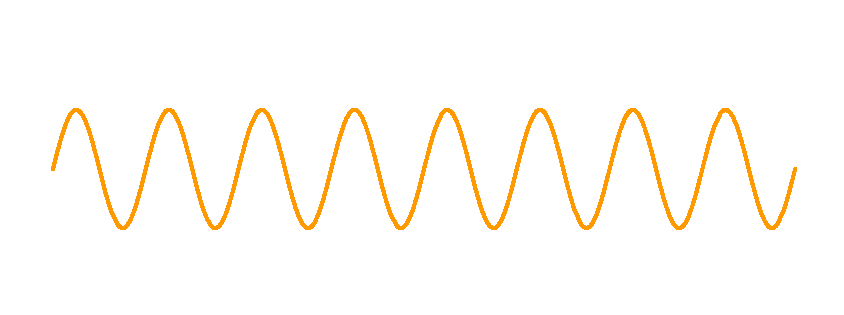
\includegraphics[width=0.9\columnwidth]{res/pdf/2/pitch/A5.eps}
				\end{figure}
			\end{column}
		\end{columns}
		\begin{columns}
			\begin{column}{0.5\textwidth}
				\centering
				\color{cyan} \href{run:res/mp3/2/pitch/A4.mp3}{A$_4$ 440 Hz}
			\end{column}
			\begin{column}{0.5\textwidth}
				\centering
				\color{cyan} \href{run:res/mp3/2/pitch/A5.mp3}{A$_5$ 880 Hz}
			\end{column}
		\end{columns}
		%Split 'columns' environment, rather than merging into one. Then there are less margins!
		음정이 연관되는 예시로는 멜로디, 화음, 튜닝 등이 있습니다.
	\end{frame}
	
	\begin{frame}
		\frametitle{Section \ref{sec:music} : 음악이란?}
		\framesubtitle{음정(timbre)}
		같은 음이라도 피아노 소리랑 사람의 목소리랑 피콜로의 소리는 다릅니다. 이는 주파수의 파형(맵시)가 다르기 때문입니다.
		\begin{columns}
			\begin{column}{0.5\textwidth}
				\centering
				\noindent
				\begin{figure}[h!]
					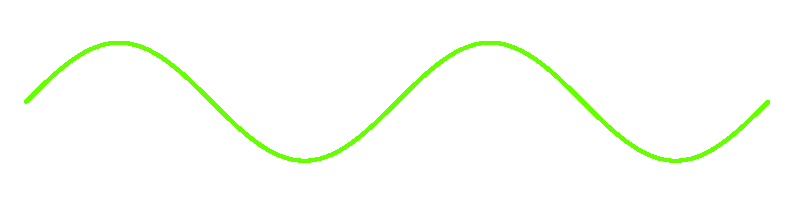
\includegraphics[width=0.9\columnwidth]{res/pdf/2/timbre/sine.eps}
				\end{figure}
				\noindent
			\end{column}
			\begin{column}{0.5\textwidth}
				\centering
				\begin{figure}[h!]
					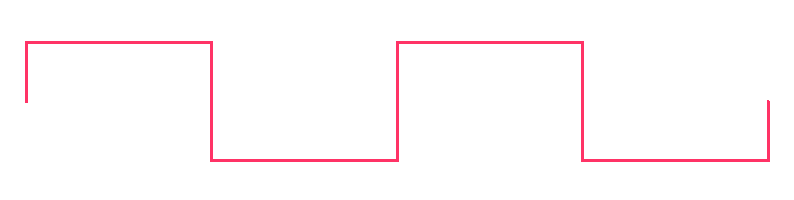
\includegraphics[width=0.9\columnwidth]{res/pdf/2/timbre/square.eps}
				\end{figure}
			\end{column}
		\end{columns}
		\begin{columns}
			\begin{column}{0.5\textwidth}
				\centering
				\color{cyan} \href{run:res/mp3/2/timbre/sine.mp3}{C$_5$ sine waveform}
			\end{column}
			\begin{column}{0.5\textwidth}
				\centering
				\color{cyan} \href{run:res/mp3/2/timbre/square.mp3}{C$_5$ square waveform}
			\end{column}
		\end{columns}
		악기 등의 음색을 합성해내는 것은, 요즘은 훌륭한 신디사이저와 {\bf 푸리에 변환}의 도움으로 그럴 듯 하게 되는 경우도 있습니다.
	\end{frame}
	
	\begin{frame}
		\frametitle{Section \ref{sec:music} : 음악이란?}
		\framesubtitle{세기(loudness)}
		소리는 세기를 가집니다. 얼마나 크고 작게 들리는지에 대한 것으로, 파장의 진폭(amplitude)과 관련이 있습니다. \\
		\vskip 1pc
		\centering{\color{cyan} \href{run:res/mp3/2/loudness/surprise.mp3}{Symphony No. 94 (Haydn)}}\\
		\flushleft
		이 세기는 셈여림({\it e.g. piano, forte})과 아티큘레이션({\it e.g. staccato})과 관련이 있습니다.
	\end{frame}
	
	\begin{frame}
		\frametitle{Section \ref{sec:music} : 음악이란?}
		\framesubtitle{길이(duration)}
		같은 음높이에 같은 음정에 같은 세기라도 지속되는 길이에 따라 소리는 달라집니다. 이건 굳이 mp3 파일로 만들 필요도 없을 것 같네요. 다만 이 길이와 관련있는 개념들도 많습니다. 곡의 빠르기(tempo)라든지, 박자(beat)라든지......
	\end{frame}
	
	\subsection{The importance of harmony}
	\begin{frame}
		\frametitle{Section \ref{sec:music} : 음악이란?}
		\framesubtitle{......그래서요?}
		저렇게 소리의 요소들을 통해서 대부분의 사람들이 음악으로 만들어내고자 하는 것은 바로 {\bf 조화(harmony)}입니다. 의도적으로 불협화음을 넣는 수도 있지만, 음악은 {\bf 조화롭게} 느껴지는 경우가 대부분입니다.
	\end{frame}
	
	\begin{frame}
		\frametitle{Section \ref{sec:music} : 음악이란?}
		\framesubtitle{조화로운 음악}
		이 성질은 상당히 중요합니다. 왜냐하면 귀에 조화롭게 들리는 음들로 화음이나 진행들을 주로 진행해 나가려 하기 때문이죠. 물론, 모든 음의 조합이 조화롭게 들리지는 않겠지요. 다음 교가를 한 번 들어보세요.
		\vskip 1pc
		\begin{columns}
			\begin{column}{0.5\textwidth}
				\centering
				\color{cyan} \href{run:res/mp3/2/harmony/school.mp3}{Normal school song}
			\end{column}
			\begin{column}{0.5\textwidth}
				\centering
				\color{cyan} \href{run:res/mp3/2/harmony/school_weird.mp3}{Normal school song?}
			\end{column}
		\end{columns}
	\end{frame}
	
	\begin{frame}
		\frametitle{Section \ref{sec:music} : 음악이란?}
		\framesubtitle{그래서 조화로운 게 뭔가요?}
		문제는 `조화롭다'의 기준이 직관에 의존할 수 밖에 없다는 것입니다. 그렇기 때문에 무엇이 조화로운지 스스로 못 느끼는 사람들도 많으며, 무엇이 조화로운 지는 알더라도 왜 조화로운지 모르는 사람도 많습니다. 그리고 이것을 이론적으로 연구한 것이 바로 {\bf 화성학}이 되는 것이죠.
	\end{frame}
	
	\section{Section 3 : Harmony}\label{sec:harmony}
	\subsection{Discussion about harmony}
	\begin{frame}
		\frametitle{Section \ref{sec:harmony} : 화성학이란?}
		\framesubtitle{화성학의 정의}
		\begin{definition}[화성학, Study of Harmony]
			\begin{itemize}
				\item 화음에 기초를 두고 그 구성, 연결, 방법 및 음 조직을 연구하는 분야. - 표준국어대사전
			\end{itemize}
		\end{definition}
	\end{frame}
	
	\begin{frame}
		\frametitle{Section \ref{sec:harmony} : 화성학이란?}
		\framesubtitle{조화에 대한 연구, 화성학}
		사람들은 화음, 즉 음을 여러 개 쌓아놓은 것에 대해서 수많은 연구를 했습니다. 그것이 바로 화성학입니다. 어떠한 것이 조화로운지는 시대에 따라 달라왔지만, 크게 화성학은 2가지로 나눌 수 있습니다. 이가 바로 {\bf 클래식 화성학}과 {\bf 실용화성학}입니다.
	\end{frame}
	
	\begin{frame}
		\frametitle{Section \ref{sec:harmony} : 화성학이란?}
		\framesubtitle{클래식 화성학(Classical Harmony)}
		클래식 화성학이 원래는 기존의 화성학이었습니다. 흔히 클래식, 즉 고전음악이라 불리는 곡들에게 적용되는 규칙이라 할 수 있죠. 그러나 엄격합니다. 제한되는 게 많거든요({\it e.g. 병행 8도}). 진행이든, 반주든, 코드든 말이죠. 이는 기본적으로 클래식 화성학이 각 음(note)에 초점을 두었기 때문에 그렇습니다. 
	\end{frame}
	
	\begin{frame}
		\frametitle{Section \ref{sec:harmony} : 화성학이란?}
		\framesubtitle{실용화성학(Jazz Harmony)}
		반면 실용화성학(재즈 화성학이라고도 합니다)은 그런 것에서 자유로운 감이 있습니다. 클래식 화성학에서 파생되었지만, `실용'이라는 이름에 걸맞게, 각종 예외를 다 허용하고, 초점을 화음(chord)에 맞추었기 때문입니다.
	\end{frame}
	
	\subsection{Plans}
	\begin{frame}
		\frametitle{Section \ref{sec:harmony} : 화성학이란?}
		\framesubtitle{그래서 뭘 배울 건가요?}
		실용화성학의 기본적인 개념은 일단 클래식 화성학과 일치하기에 일단 기본적인 내용은 클래식 화성학에서 시작할 겁니다만, 일단 제가 생각하기에 정말 필요하다는 것 위주로 골라서 설명할 예정입니다.
	\end{frame}
	
	\begin{frame}
		\frametitle{Section \ref{sec:harmony} : 화성학이란?}
		\framesubtitle{이것만 알면 되나요?}
		사실 이런 건 교재나 레슨, 강의 등을 들으면서 배우는 것이 제일 낫습니다. 그 쪽이 더 정확하고 체계적이기 때문이죠.\\
		그리고 음악를 구성하는 학문은 이거 말고도 많이 있습니다. 음악사학이라든지, 음향학이라든지, 대위법이라든지......배울 건 많으니 걱정하진 마세요.
	\end{frame}
	
	\begin{frame}
		\frametitle{Section \ref{sec:harmony} : 화성학이란?}
		\framesubtitle{드디어 화성학 강의를 시작하는 건가요?}
		그러고 싶지만......화성학을 설명하기 위해 필요한 내용들이 있습니다. 바로 (현대 음악) {\bf 기보법}입니다. 좀 많은 내용을 다루고 가야 하거든요.
	\end{frame}
	
	\section{Section 4 : Musical Notations}\label{sec:notations}
	\subsection{Basic signatures about modern musical notations}
	\begin{frame}
		\frametitle{Section \ref{sec:notations} : 기보법}
		\framesubtitle{기보법이 뭔가요?}
		\begin{definition}[기보법, Musical Notation]%記譜法 behaving odd
			\begin{itemize}
				\item 음악의 연주나 발표, 보존, 학습 따위를 목적으로 일정한 약속이나 규칙에 따라 기호를 써서 악곡을 기록하는 방법. \\- 표준국어대사전
			\end{itemize}
		\end{definition}
	\end{frame}
	
	\begin{frame}
		\frametitle{Section \ref{sec:notations} : 기보법}
		\framesubtitle{갑자기 기보법은 왜 나오죠?}
		......사실 기보법은 음악을 표현하기 위해 사용하는 표기법을 다루는 학문입니다. 화성학의 한 갈래는 아니죠. 다만 이 기보법을 통해 악보에 음악을 진행해 나가는 경우가 많습니다. 그리고 여기서 이야기하는 기보법은 정간보나 고대의 음악이 아닌, 현대 음악들에 대한 이야기입니다. {\bf 오선지} 위에 하는 그거요.
	\end{frame}
	
	\begin{frame}
		\frametitle{Section \ref{sec:notations} : 기보법}
		\framesubtitle{전 이런 거 다 알고 있는데요.}
		전 학교 다니면서 이 정도는 다 알고 있을 줄 알았는데, 생각보다 중학교 음악 시간에 집중하지 않은 사람들이 많더군요. 용어들도 그렇고요. 때문에 이 장에서 그러한 것들을 다루고자 합니다. 좀 많겠지만요.
	\end{frame}
	
	\begin{frame}
		\frametitle{Section \ref{sec:notations} : 기보법}
		\framesubtitle{오선보(staff)}
		그래도 오선보가 뭔진 아시죠? 이겁니다.
		\begin{figure}[h!]
			\centering
			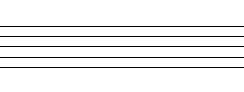
\includegraphics[width=0.5\columnwidth]{res/pdf/4/staff/staff.pdf}
		\end{figure}
		\vskip -1pc
		5개의 수평선과 4개의 공백으로 이루어져 있으며, 위치에 따라 연주 시간과 음높이가 달라집니다.
	\end{frame}
	
	\begin{frame}
		\frametitle{Section \ref{sec:notations} : 기보법}
		\framesubtitle{음자리표(clef)}
		하지만 저 오선보만 있으면 어느 높이가 어느 음인지 알 수 없습니다. 이 기준을 세워주는 기호가 바로 {\bf 음자리표(clef)}입니다. 기준은 {\color{cyan} \href{run:res/mp3/4/clef/C4.mp3}{C$_4$(261.6 Hz)}} 입니다.
		\begin{columns}
			\begin{column}{0.3\textwidth}
				\centering
				\noindent
				\begin{figure}[h!]
					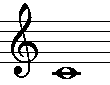
\includegraphics[width=0.7\columnwidth]{res/pdf/4/clef/g_clef.pdf}
				\end{figure}
				%\small 높은음자리표(G clef)
			\end{column}
			\begin{column}{0.3\textwidth}
				\centering
				\noindent
				\begin{figure}[h!]
					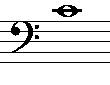
\includegraphics[width=0.7\columnwidth, trim=0 0 0 0.3pc]{res/pdf/4/clef/f_clef.pdf}
				\end{figure}
				%\vskip 0.4pc
				%\small 낮은음자리표(F clef)
			\end{column}
			\begin{column}{0.3\textwidth}
				\centering
				\noindent
				\begin{figure}[h!]
					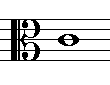
\includegraphics[width=0.7\columnwidth]{res/pdf/4/clef/c_clef.pdf}
				\end{figure}
				%\small 가온음자리표(C clef)
			\end{column}
		\end{columns}
		\begin{columns}
			\begin{column}{0.3\textwidth}
				\centering
				\small 높은음자리표(G clef)
			\end{column}
			\begin{column}{0.3\textwidth}
				\centering
				\small 낮은음자리표(F clef)
			\end{column}
			\begin{column}{0.3\textwidth}
				\centering
				\small 가온음자리표(C clef)
			\end{column}
		\end{columns}
		음자리표는 기본적으로 오선보 각 줄의 가장 좌측에 위치하며, 음자리표가 바뀌지 않는 이상 그 외에서는 나타나지 않습니다.
	\end{frame}
	
	\begin{frame}
		\frametitle{Section \ref{sec:notations} : 기보법}
		\framesubtitle{박자표(time signature)}
		이에 비해 박자표는 한 마디(measure, 악곡의 가장 작은 단위)가 몇 박자로 이루어져 있는지를 지시하는 기호입니다.
		\begin{figure}[!h]
			\centering{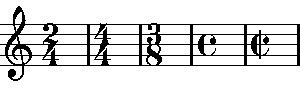
\includegraphics[width=0.7\textwidth]{res/pdf/4/time/time.pdf}}
		\end{figure}
		2/4의 경우 4분음표 2개가 한 마디, 3/8의 경우 8분음표 3개가 한 마디인 식입니다. 마디의 구분은 세로줄로 하며, 마지막 2개는 각각 4/4, 2/2를 나타내는 또 다른 기호입니다.
	\end{frame}
	
	\begin{frame}
		\frametitle{Section \ref{sec:notations} : 기보법}
		\framesubtitle{조표(key signature)}
		조표는 조성(tonality)을 결정짓는 기호입니다. 좀 간단히 말하자면, {\bf 이 곡이 무슨 장조이고 무슨 단조인지를 결정하는 기호입니다.} 다음은 간단한 예시입니다.
		\begin{figure}[!h]
			\centering{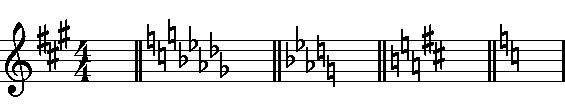
\includegraphics[width=0.9\textwidth]{res/pdf/4/key/transpose.pdf}}
		\end{figure}
		조표에 관한 더 자세한 내용은 7장에서 설명하겠습니다. 그래도 {\bf 음자리표-조표-박자표}의 순서는 알고 계세요.
	\end{frame}
	
	\subsection{Solfège}
	\begin{frame}
		\frametitle{Section \ref{sec:notations} : 기보법}
		\framesubtitle{도레미파솔라시도}
		\flushleft
		아무튼 이러한 악보를 보면서 여러분들은 `도레미파솔라시도'라는 것을 들어보셨을 겁니다. 이렇게 말이죠.\\
		\begin{figure}[!h]
			\centering
			{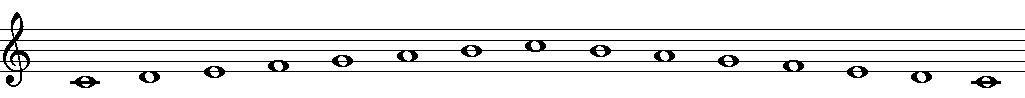
\includegraphics[width=\textwidth]{res/pdf/4/syllable/doremi.pdf}}
		\end{figure}
		\centering
		\color{cyan}\href{run:res/mp3/4/syllable/doremi.mp3}{직접 들어 보세요.}	
	\end{frame}
	
	\begin{frame}
		\frametitle{Section \ref{sec:notations} : 기보법}
		\framesubtitle{도레미파솔라시도?}
		\flushleft
		방금 전 들으신 건 자연스럽게 `도레미파솔라시도'라는 말이 나왔을 겁니다. 그러면 이건 어떻게 부르실 건가요?\\
		\begin{figure}[!h]
			\centering
			{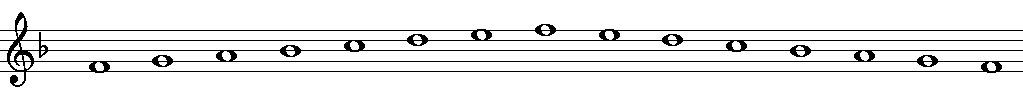
\includegraphics[width=\textwidth]{res/pdf/4/syllable/doremi_F.pdf}}
		\end{figure}
		\centering
		\color{cyan}\href{run:res/mp3/4/syllable/doremi_F.mp3}{역시 직접 들어 보세요.}	
	\end{frame}
	
	\begin{frame}
		\frametitle{Section \ref{sec:notations} : 기보법}
		\framesubtitle{이건 파솔라시도레미파 아닌가요?}
		파솔라시도레미파요? 시는 반음 낮은 시 플랫이라고요? 결론부터 말하겠습니다. \bf 이것도 도레미파솔라시도입니다. 	
	\end{frame}
	
	\begin{frame}
		\frametitle{Section \ref{sec:notations} : 기보법}
		\framesubtitle{이게 파가 아니라 왜 도인가요.}
		그 이유는 {\bf 계이름}의 정의에서 찾아볼 수 있습니다.
		\begin{definition}[계이름, syllable name]
			\begin{itemize}
				\item 음계를 이루는 자리의 이름. 각 음의 높이의 상대적인 관계를 나타내는 것으로, 절대 음높이를 나타내는 음이름과 구별된다. - 표준국어대사전
				\item In Movable do, or tonic sol-fa, each syllable corresponds to a scale degree. - Wikipedia
			\end{itemize}
		\end{definition}
		서양 음악의 `도, 레, 미, 파, 솔, 라, 시'가 여기에 해당하며, 여기서 기준이 되는 음은 (나중에 배울) {\it 으뜸음}이라는 녀석입니다.
	\end{frame}
	
	\begin{frame}
		\frametitle{Section \ref{sec:notations} : 기보법}
		\framesubtitle{그러면 절대적인 기준은 없나요?}
		당연히 있죠. 그것이 바로 {\bf 음이름}입니다.
		\begin{definition}[음이름, pitch name]
			\begin{itemize}
				\item 개개 음의 절대적인 높이를 가리키기 위하여 음마다 붙이는 이름. - 표준국어대사전
				\item In Fixed do, each syllable corresponds to the name of a note. - Wikipedia
			\end{itemize}
		\end{definition}
		서양 음악에서는 `C, D, E, F, G, A, B', 우리나라에서는 `다, 라, 마, 바, 사, 가, 나'의 일곱 문자와 샤프($\sharp$), 플랫($\flat$) 등을 이용하여 나타냅니다.
	\end{frame}
	
	\begin{frame}
		\frametitle{Section \ref{sec:notations} : 기보법}
		\framesubtitle{헷갈리네요.}
		\flushleft
		음이름의 기준을 잡겠습니다.
		\begin{figure}[!h]
			\centering
			{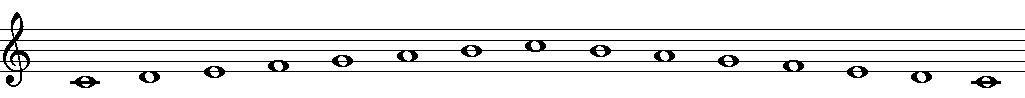
\includegraphics[width=\textwidth]{res/pdf/4/syllable/doremi.pdf}}
		\end{figure}
		처음 8개 음의 음이름은 다-라-마-바-사-가-나-다이며, C$_4$-D$_4$-E$_4$-F$_4$-G$_4$-A$_4$-B$_4$-C$_5$로 나타낼 수도 있습니다.
	\end{frame}
	
	\begin{frame}
		\frametitle{Section \ref{sec:notations} : 기보법}
		\framesubtitle{그러면 그 다음 거는요?}
		\flushleft
		바장조의 경우군요. (장조/단조 등의 조성을 이야기할 때 음이름을 쓴다는 것을 눈치채셨나요?)
		\begin{figure}[!h]
			\centering
			{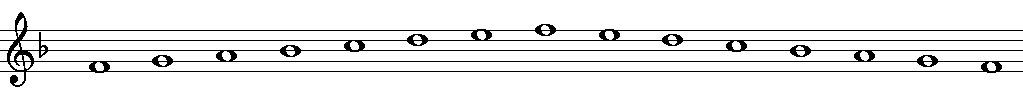
\includegraphics[width=\textwidth]{res/pdf/4/syllable/doremi_F.pdf}}
		\end{figure}
		처음 8개 음의 음이름은 바-사-가-내림나-다-라-마-바이며, F$_4$-G$_4$-A$_4$-B$\flat_4$-C$_5$-D$_5$-E$_5$-F$_5$로 나타낼 수도 있습니다.\\
		하지만 두 경우 모두 계이름은 도레미파솔라시도입니다.
	\end{frame}
	
	\begin{frame}
		\frametitle{Section \ref{sec:notations} : 기보법}
		\framesubtitle{계이름이랑 음이름이랑 별로 구분 안하고 쓰지 않나요?}
		실제로 많이 혼용되어서 쓰이고 있습니다. 특히 음이름을 써야 할 곳에 (즉 절대적인 음을 매겨야 할 때) 계이름을 쓰는 경우가 많습니다. 그러나 화성학에서는 기본적으로 음들간의 상대적인 관계를 절대적인 수치로 나타내므로 음이름을 쓰는 경우가 많습니다. {\bf 그 기준이 주로 {\color{cyan} \href{run:res/mp3/2/pitch/A4.mp3}{A$_4$를 440 Hz로 잡는 것입니다.}}} 일부 오케스트라에서는 튜닝을 달리 하기도 하지만요.
	\end{frame}
	
	\begin{frame}
		\frametitle{Section \ref{sec:notations} : 기보법}
		\framesubtitle{뭔가 잘 이해가 안 되네요.}
		맞는 말입니다. 이걸 보면서 음이름과 계이름을 배우는 것도 좋지만, 직접 피아노를 연주하시든지 MuseScore로 음을 찍어 가시든지 해 보세요. 음은 글을 본다고 해서 이해되는 것이 아닙니다. {\bf 글은 시각적인 자료이고 음은 청각적인 자료이니까요.}\\
		그래도 이런 Solfège(솔페이지, 음을 읽는 것을 뜻합니다)가 기본적으로 되야, 5장 이후의 내용이 그나마 이해가 될 겁니다. 그러면 다시 기보법으로 돌아가겠습니다.
	\end{frame}
	\subsection{Basic concepts about notes/rests}
	\begin{frame}
		\frametitle{Section \ref{sec:notations} : 기보법}
		\framesubtitle{음표(note)}
		이제야 설명하네요. 음을 나타내는 음표입니다. 음표의 가로 위치는 음의 길이를, 세로 위치는 음의 음높이를 나타내는데 음높이는 방금 전까지 이야기 했습니다. 그러면 음의 길이를 이야기할 차례겠지요.
	\end{frame}
	
	\begin{frame}
		\frametitle{Section \ref{sec:notations} : 기보법}
		\framesubtitle{음표와 쉼표(note)}
		한 마디 안에는 정확히 박자표에서 지시한 만큼의 박자가 들어가야 합니다. 못갖춘마디 등을 제외하면 말이죠. 이 중 음표는 어떠한 음을 얼마나 연주할지, 쉼표는 얼마나 연주를 하지 않을지를 나타냅니다.\\
	\end{frame}
	
	\begin{frame}
		\frametitle{Section \ref{sec:notations} : 기보법}
		\framesubtitle{음표(note)}
		\vskip -1pc
		\begin{columns}
			\begin{column}{0.33\textwidth}
				\centering
				\noindent
				\begin{figure}[h!]
					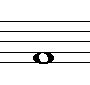
\includegraphics[width=0.7\columnwidth]{res/pdf/4/note/whole.pdf}
				\end{figure}
			\end{column}
			\begin{column}{0.33\textwidth}
				\centering
				\noindent
				\begin{figure}[h!]
					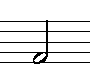
\includegraphics[width=0.7\columnwidth]{res/pdf/4/note/half.pdf}
				\end{figure}
			\end{column}
			\begin{column}{0.33\textwidth}
				\centering
				\noindent
				\begin{figure}[h!]
					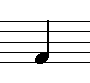
\includegraphics[width=0.7\columnwidth]{res/pdf/4/note/quarter.pdf}
				\end{figure}
			\end{column}
		\end{columns}
		\vskip -1pc
		\begin{columns}
			\begin{column}{0.33\textwidth}
				\centering
				\small 온음표,\\whole note, 4박자
			\end{column}
			\begin{column}{0.33\textwidth}
				\centering
				\small 2분음표,\\half note, 2박자
			\end{column}
			\begin{column}{0.33\textwidth}
				\centering
				\small 4분음표,\\quarter note, 1박자
			\end{column}
		\end{columns}
		\vskip -1pc
		\begin{columns}
			\begin{column}{0.33\textwidth}
				\centering
				\noindent
				\begin{figure}[h!]
					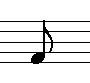
\includegraphics[width=0.7\columnwidth]{res/pdf/4/note/eighth.pdf}
				\end{figure}
			\end{column}
			\begin{column}{0.33\textwidth}
				\centering
				\noindent
				\begin{figure}[h!]
					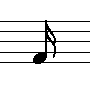
\includegraphics[width=0.7\columnwidth]{res/pdf/4/note/sixteenth.pdf}
				\end{figure}
			\end{column}
			\begin{column}{0.33\textwidth}
				\centering
				\noindent
				\begin{figure}[h!]
					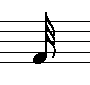
\includegraphics[width=0.7\columnwidth]{res/pdf/4/note/thirty-second.pdf}
				\end{figure}
			\end{column}
		\end{columns}
		\vskip -1pc
		\begin{columns}
			\begin{column}{0.33\textwidth}
				\centering
				\small 8분음표,\\eighth note, $\frac{1}{2}$박자
			\end{column}
			\begin{column}{0.33\textwidth}
				\centering
				\small 16분음표,\\sixteenth note, $\frac{1}{4}$박자
			\end{column}
			\begin{column}{0.33\textwidth}
				\centering
				\small 32분음표,\\thirty-second note,\\$\frac{1}{8}$박자
			\end{column}
		\end{columns}
	\end{frame}
	
	\begin{frame}
		\frametitle{Section \ref{sec:notations} : 기보법}
		\framesubtitle{쉼표(rest)}
		\vskip -1pc
		\begin{columns}
			\begin{column}{0.33\textwidth}
				\centering
				\noindent
				\begin{figure}[h!]
					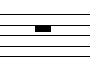
\includegraphics[width=0.7\columnwidth]{res/pdf/4/rest/whole.pdf}
				\end{figure}
			\end{column}
			\begin{column}{0.33\textwidth}
				\centering
				\noindent
				\begin{figure}[h!]
					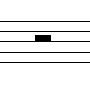
\includegraphics[width=0.7\columnwidth]{res/pdf/4/rest/half.pdf}
				\end{figure}
			\end{column}
			\begin{column}{0.33\textwidth}
				\centering
				\noindent
				\begin{figure}[h!]
					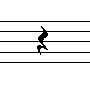
\includegraphics[width=0.7\columnwidth]{res/pdf/4/rest/quarter.pdf}
				\end{figure}
			\end{column}
		\end{columns}
		\vskip -1pc
		\begin{columns}
			\begin{column}{0.33\textwidth}
				\centering
				\small 온쉼표,\\whole rest, 4박자
			\end{column}
			\begin{column}{0.33\textwidth}
				\centering
				\small 2분쉼표,\\half rest, 2박자
			\end{column}
			\begin{column}{0.33\textwidth}
				\centering
				\small 4분쉼표,\\quarter rest, 1박자
			\end{column}
		\end{columns}
		\vskip -1pc
		\begin{columns}
			\begin{column}{0.33\textwidth}
				\centering
				\noindent
				\begin{figure}[h!]
					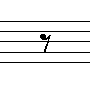
\includegraphics[width=0.7\columnwidth]{res/pdf/4/rest/eighth.pdf}
				\end{figure}
			\end{column}
			\begin{column}{0.33\textwidth}
				\centering
				\noindent
				\begin{figure}[h!]
					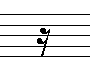
\includegraphics[width=0.7\columnwidth]{res/pdf/4/rest/sixteenth.pdf}
				\end{figure}
			\end{column}
			\begin{column}{0.33\textwidth}
				\centering
				\noindent
				\begin{figure}[h!]
					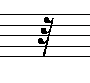
\includegraphics[width=0.7\columnwidth]{res/pdf/4/rest/thirty-second.pdf}
				\end{figure}
			\end{column}
		\end{columns}
		\vskip -1pc
		\begin{columns}
			\begin{column}{0.33\textwidth}
				\centering
				\small 8분쉼표,\\eighth rest, $\frac{1}{2}$박자
			\end{column}
			\begin{column}{0.33\textwidth}
				\centering
				\small 16분쉼표,\\sixteenth rest, $\frac{1}{4}$박자
			\end{column}
			\begin{column}{0.33\textwidth}
				\centering
				\small 32분쉼표,\\thirty-second rest,\\$\frac{1}{8}$박자
			\end{column}
		\end{columns}
	\end{frame}
	
	\begin{frame}
		\frametitle{Section \ref{sec:notations} : 기보법}
		\framesubtitle{음표와 쉼표(note)}
		음표와 쉼표에 쓰이는 몇 가지 대표적인 추가 표기법들은 다음과 같습니다. 설명은 생략하겠습니다.
		\begin{itemize}
			\item 붙임줄/이음줄(tie/slur)
			\item 글리산도/포르타멘토(glissando/portamento)
			\item 잇단음표(tuplet)
			\item 화음(chord)
			\item 아르페지오(arpeggio)
		\end{itemize}
	\end{frame}
	
	\begin{frame}
		\frametitle{Section \ref{sec:notations} : 기보법}
		\framesubtitle{임시표(accidental)}
		조표랑 똑같은 기호($ \sharp $, $ \flat $, $ \natural $)을 사용합니다. 일단 이 기호들의 역할을 알아볼까요?
		\begin{itemize}
			\item $ \sharp $(sharp), 음을 반음 올립니다.
			\item $ \flat $(flat), 음을 반음 내립니다.
			\item $ \natural $(natural), 임시표에 의해 변한 음을 원래대로 되돌립니다.
			\item \doubleflat(double flat), 음을 온음 내립니다.
			\item \doublesharp(double sharp), 음을 온음 올립니다.
		\end{itemize}
		임시표의 효력은 {\bf 그 마디에 한합니다}. 조표와의 차이죠.
	\end{frame}
	
	\begin{frame}
		\frametitle{Section \ref{sec:notations} : 기보법}
		\framesubtitle{......그런데 온음 반음이 뭔가요.}
		음......난감한 질문이군요. 다음 악보를 보시죠.
		\begin{figure}
			\centering
			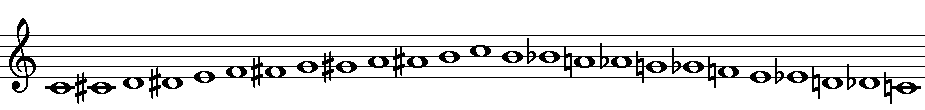
\includegraphics[width=\textwidth]{res/pdf/4/scale/chromatic.pdf}
		\end{figure}
		\centering{\color{cyan} \href{run:res/mp3/4/scale/chromatic.mp3}{한 번 들어보세요.}}
	\end{frame}
	
	\begin{frame}
		\frametitle{Section \ref{sec:notations} : 기보법}
		\framesubtitle{도레미파솔라시도는 아니네요.}
		그렇습니다. 도레미파솔라시도는 아니죠. 이건 건반악기({\it e.g. 피아노}) 등의 예시를 보는 것이 이해가 가장 잘 됩니다. 건반악기는 다음과 같이 구성이 되어 있습니다.
		\begin{figure}
			\centering
			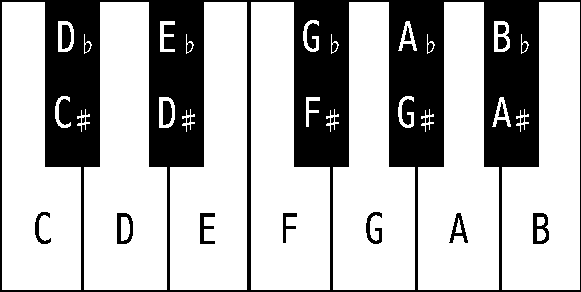
\includegraphics[width=0.9\textwidth]{res/pdf/4/scale/keys.pdf}
		\end{figure}
	\end{frame}
	
	\begin{frame}
		\frametitle{Section \ref{sec:notations} : 기보법}
		\framesubtitle{그런가요......}
		자세한 내용은 7장에서 설명할 것 같으니, 여기서는 간략히만 설명하겠습니다. 방금 전 연주했던 음은 C$_4 $부터 C$_5 $까지 {\bf 반음}씩 올라가는 음계입니다. 건반악기에서 인접한 흰 건반과 검은 건반이 서로 `반음' 관계에 있는 것이죠. 그리고 E-F, B-C간의 간격도 반음입니다. 온음은 반음 2개의 간격이고요.
	\end{frame}
	
	\begin{frame}
		\frametitle{Section \ref{sec:notations} : 기보법}
		\framesubtitle{어렵네요.}
		온음 반음은 그래도 음악 같은 걸 듣다 보면 쉽게 와닿는 개념 중 하나일 겁니다. {\bf 그러나 꼭 알아둬야 하는 개념이기도 합니다.}\\
		아무튼 여기까지가 정말 기본적인 기보법과 음악 상식이었습니다. 뭔가 부족하다 싶은 분들은  
		{\color{orange}{\href{https://musescore.org/}{MuseScore}}} 같은 프로그램을 설치하시거나 {\color{cyan}{\href{https://en.wikipedia.org/wiki/List_of_musical_symbols}{이 Wikipedia 문서}}}를 읽어보세요. 또, 실제 악보를 보는 것도 도움이 많이 됩니다.
	\end{frame}
	
	%Finally it is over! AWWWWWWWWW YEAHHHHHHHHHHH
	
	\section{Section 5 : Musical Temperament}\label{sec:temperament}
	\subsection{Definition of temperament}
	\begin{frame}
		\frametitle{Section \ref{sec:temperament} : 음률}
		\framesubtitle{음률의 정의}
		\ref{sec:temperament}장에서 다룰 내용은 음률입니다.
		\begin{definition}[음률, 音律, Temperament]
			\begin{itemize}
				\item 소리와 음악의 가락. - 표준국어대사전
			\end{itemize}
		\end{definition}
	\end{frame}
	
	\begin{frame}
		\frametitle{Section \ref{sec:temperament} : 음률}
		\framesubtitle{음률의 정의}
		표준국어대사전의 정의가 너무 간단하군요. 음률을 조금 더 풀어서 설명하자면, {\bf 음악에 사용되는 음높이들의 상대적인 관계}입니다. C,D,E 내지는 다,라,마로 음이름은 만들었지만 어떤 음이 이런 음들인지는 규칙을 정해야 하기 때문입니다.
	\end{frame}
	
	\begin{frame}
		\frametitle{Section \ref{sec:temperament} : 음률}
		\framesubtitle{음률이라......}
		앞으로도 계속 할 말이지만 음은 주파수를 가진다는 것과 음악의 기본적인 취지는 조화로움이라는 것을 잊지 마세요. 옛날부터 사람들은 음의 관계를 예쁘게 만드려고 노력했거든요. 그러한 시도는 {\bf 순정률}의 개발로 이어졌습니다.
	\end{frame}
	
	\begin{frame}
		\frametitle{Section \ref{sec:temperament} : 음률}
		\framesubtitle{순정률이란?}
		순정률의 정의는 대단히 간단합니다. {\bf 음 사이의 비가 유리수인 음률}을 순정률이라고 합니다. 그 유리수가 간단한 정수비로 나타나면 더욱 좋겠죠. 그런 관점에서 순정률의 초석을 다져놓은 사람이 바로 {\bf 피타고라스}입니다.
	\end{frame}
	
	\subsection{Pythagorean tuning}
	\begin{frame}
		\frametitle{Section \ref{sec:temperament} : 음률}
		\framesubtitle{피타고라스 음률(Pythagorean tuning)}
		피타고라스 음률은 정말 간단합니다. 다음 2개의 규칙만 따르면 되니까요.
		\begin{itemize}
			\item 1. 도와 높은 도, 즉 옥타브의 주파수비는 $ 1:2 $이다. 
			\item 2. 도와 솔의 주파수비는 $ 2:3 $이다.
		\end{itemize}
	\end{frame}
	
	\begin{frame}
		\frametitle{Section \ref{sec:temperament} : 음률}
		\framesubtitle{피타고라스 음률(Pythagorean tuning)}
		저게 답니다. 그럼에도 불구하고 효과적이었습니다. 왜냐하면 얼추 조화롭다고 여겨졌기 때문이고, 저 두 규칙은 모두 합당하다고 여겨졌기 때문입니다. 아무튼 저 방식을 적용해서 각 음별 주파수비를 구하면 다음과 같습니다. {\color{cyan}\href{run:res/mp3/5/pythagorean/p_temperament.mp3}{한번 들어 보세요.}}
		\begin{table}[!h]
			\centering
			\begin{tabular}{|c|c|c|c|c|c|c|c|c|c|c|c|c|}
				\hline
				C & C$\sharp$ & D & D$\sharp$ & E & F & F$\sharp$ & G & G$\sharp$ & A & A$\sharp$ & B & C \\ \hline
				$\frac{1}{1}$ &  $\frac{256}{243}$  & $\frac{9}{8}$ & $\frac{32}{27}$ & $\frac{81}{64}$ & $\frac{4}{3}$ & $\frac{1024}{729}$ & $\frac{3}{2}$ & $\frac{128}{81}$ & $\frac{27}{16}$ & $\frac{16}{9}$ & $\frac{243}{128}$ & $\frac{2}{1}$ \\ \hline
			\end{tabular}
		\end{table}
		뭐 이런 건 영재성 검사 퀴즈에도 종종 쓰이죠.
	\end{frame}
	
	\begin{frame}
		\frametitle{Section \ref{sec:temperament} : 음률}
		\framesubtitle{피타고라스 콤마(Pythagorean comma)}
		하지만 저 음률에는 치명적인 결점이 있습니다. 바로 {\bf 피타고라스 콤마}라 불리는 현상이죠. 이론상 도-솔의 관계로 7반음을 올라가는 것을 12번 반복하고 이를 다시 7옥타브만큼 내리면 원래의 음으로 돌아와야 하는데 그렇지 않습니다. 왜냐하면 $$ \left(\dfrac{3}{2}\right )^{12}\cdot\left(\dfrac{1}{2}\right)^7=\dfrac{531441}{524288}\simeq 1.014$$이기 때문입니다. {\color{cyan}\href{run:res/mp3/5/pythagorean/comma.mp3}{그 차이를 느껴보세요.}} 첫 번째 음은 C$_4$입니다. 반면 두 번째 음은 C$_4 $보다 주파수가 약 1.014배 높습니다.
	\end{frame}
	
	\begin{frame}
		\frametitle{Section \ref{sec:temperament} : 음률}
		\framesubtitle{피타고라스 음률의 또다른 단점}
		그뿐만이 아닙니다. 피타고라스 음률은 반음 사이의 주파수비가 {\bf 일정하지 않다는 것도 문제였습니다.} 이는 협주를 하거나 조를 옮기려고 할 때 불협화음을 수반하는 원인이 되었습니다. \\
		같은 음을 내고 있는데 분명히 다른 주파수를 가지니까요.
	\end{frame}
	
	\begin{frame}
		\frametitle{Section \ref{sec:temperament} : 음률}
		\framesubtitle{비단 피타고라스 음률만의 문제는 아닌......}
		사실 이런 문제점은 다른 순정률에서도 피할 수 있는 문제는 아니었습니다. 순정률은 분명 유리수 비의 특성상 조화로웠지만 필연적으로 그러한 오차가 나타났기 때문입니다. 이러한 문제점을 딛고 나타난 음률이 {\bf 평균율}입니다.
	\end{frame}
	
	\subsection{Equal temperament}
	\begin{frame}
		\frametitle{Section \ref{sec:temperament} : 음률}
		\framesubtitle{평균율(equal temperament)}
		평균율(equal temperament)은 명칭이 의미하는 것처럼, 반음 사이의 간격이 항상 일정합니다. 그 비는 정확히 $ 2^\frac{1}{12} $입니다(12개의 반음이 있기 때문입니다). 이렇게 반음 사이의 간격이 일정해지면 조를 바꿀 때 불협화음이 나지 않는다는 것과, 임의의 경우에 대해서도 음이 조화롭게 소리가 난다는 점이 있습니다. 다만 음들의 비가 유리수 비가 아니기에, 평균율은 순정률은 아닙니다.
	\end{frame}
	
	\begin{frame}
		\frametitle{Section \ref{sec:temperament} : 음률}
		\framesubtitle{순정률과 평균율}
		현대에 들어서는 평균율이 편의상 많이 쓰이기는 하지만, 순정률이 필요한 고전 음악이나 일부 악기의 튜닝은 순정률에 맞추어져 있는 경우도 있습니다. 음들 사이의 비율이 유리수비가 아니면 필연적으로 맥놀이 현상이 발생하기 때문이죠. 때문에 간단한 정수비로 이루어진 음들의 관계가 중요하게 여겨졌으며, 이에 대한 이야기를 \ref{sec:interval}장에서 이어나가겠습니다.
	\end{frame}
	
	\section{Section 6 : Interval}\label{sec:interval}
	\subsection{Definition of interval}
	\begin{frame}
		\frametitle{Section \ref{sec:interval} : 음정}
		\framesubtitle{음정의 정의}
		\begin{definition}[음정, 音程, Interval]
			\begin{itemize}
				\item 높이가 다른 두 음 사이의 간격. 서양 음악의 장음계를 기준으로 ‘도(度)’를 단위로 표시하며, 같은 수치의 도로 표시되는 음정도 완전ㆍ장ㆍ단ㆍ증ㆍ감에 의하여 크기를 구별한다. - 표준국어대사전
			\end{itemize}
		\end{definition}
	\end{frame}
	
	\begin{frame}
		\frametitle{Section \ref{sec:interval} : 음정}
		\framesubtitle{음정의 정의}
		네. 두 음 사이의 간격이 음정입니다. 이것이 왜 중요하느냐 하면 음이 여러 개 있다고 해서 다 조화롭게 들리지는 않기 때문입니다. 괜히 불협화음이란 말이 있는 것이 아니죠.
	\end{frame}
	
	\begin{frame}
		\frametitle{Section \ref{sec:interval} : 음정}
		\framesubtitle{그러면 어떤 음정이 조화롭게 들리나요?}
		\ref{sec:temperament}장에서 말한 것처럼, 간단한 정수비로 나타내지는 경우가 조화롭고 안정한 것으로 여겨집니다. \\
		그런 화음들을 {\bf 협화음(consonance)}이라고 하며, 그렇지 않고 조화롭지 않게 들리는 화음들을 {\bf 불협화음(dissonance)}라고 합니다.
	\end{frame}
	
	\begin{frame}
		\frametitle{Section \ref{sec:interval} : 음정}
		\framesubtitle{음정의 구성}
		음정은 2개의 요소로 구성되어 있습니다.
		\begin{itemize}
			\item 음정이 완전, 장, 단, 증, 감인지(quality)
			\item 음정이 몇 도 떨어져 있는지(number)
		\end{itemize}
		일단 도의 개념을 설명하겠습니다.
	\end{frame}
	
	\subsection{Examples of intervals - The Basics}
	\begin{frame}
		\frametitle{Section \ref{sec:interval} : 음정}
		\framesubtitle{도의 개념}
		다음 오선보를 한 번 봅시다. {\color{cyan}\href{run:res/mp3/6/interval/main.mp3}{한 번 들어 보세요.}}
		\begin{figure}
			\centering
			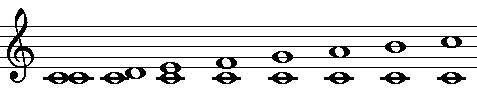
\includegraphics[width=\textwidth]{res/pdf/6/interval/diatonic.pdf}
		\end{figure}
		순서대로 각각 1도, 2도, 3도, 4도, 5도, 6도, 7도, 8도입니다. 즉 `도-레-미-파-솔-라-시-도'의 관계에서 얼마나 떨어져 있느냐로 계산하는 겁니다. 기본적으로는 이 도의 구분은 온음이지만, {\bf 반음이 그 중 몇 개가 있느냐}가 관건이 됩니다.
	\end{frame}
	
	\begin{frame}
		\frametitle{Section \ref{sec:interval} : 음정}
		\framesubtitle{완전음정(perfect interval)}
		이 중 {\color{cyan}\href{run:res/mp3/6/interval/perfect.mp3}{1도, 4도, 5도, 8도}}에 주목하시기 바랍니다. 
		\begin{figure}
			\centering
			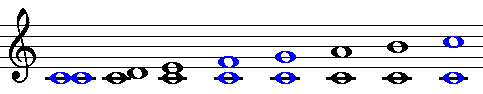
\includegraphics[width=\textwidth]{res/pdf/6/interval/perfect.pdf}
		\end{figure}
		1도, 4도, 5도, 8도는 {\bf 협화음}입니다. 대단히 안정하고 조화롭다 여겨지는 화음들인 것이죠. 그도 그럴 것이 진동수의 비가 거의 각각 1:1, 4:3, 3:2, 2:1이거든요.
	\end{frame}
	
	\begin{frame}
		\frametitle{Section \ref{sec:interval} : 음정}
		\framesubtitle{완전음정(perfect interval)}
		이 음정들을 {\bf 완전음정}이라 하며, `완전'을 앞에 붙여 말합니다. 완전4도 이런 식으로요. 더 세부적으로 분석하면 다음과 같습니다.
		\begin{table}[!h]
			\centering
			\small
			\begin{tabular}{|c|c|c|c|c|}
				\hline
				음정 & Interval & 음의 간격 & 포함된 반음 개수 & 진동수비 \\ \hline
				완전1도  &  Perfect unison  &  0반음  &  0쌍  &  1:1  \\ \hline
				완전4도  &  Perfect fourth  &  5반음  &  1쌍(미-파)  &  4:3  \\ \hline
				완전5도  &  Perfect fifth  &  7반음  &  1쌍(미-파)  &  3:2  \\ \hline
				완전8도  &  Perfect octave & 12반음  &  2쌍(미-파, 시-도)  &  2:1  \\ \hline
			\end{tabular}
		\end{table}
		`포함된 반음의 개수'는 도 기준입니다.
	\end{frame}
	
	\begin{frame}
		\frametitle{Section \ref{sec:interval} : 음정}
		\framesubtitle{장음정(major interval)}
		이번에는 {\color{orange}\href{run:res/mp3/6/interval/major.mp3}{2도, 3도, 6도, 7도}}에 주목하시기 바랍니다. 
		\begin{figure}
			\centering
			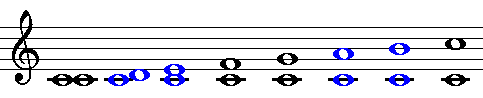
\includegraphics[width=\textwidth]{res/pdf/6/interval/major.pdf}
		\end{figure}
		이중 3도, 6도는 {\bf 협화음}입니다. 완전음정까지는 아니지만 어느 정도 조화롭다는 의미입니다. 반면 2도와 7도는 {\bf 불협화음}으로 여겨집니다. 물론, 시대와 문화에 따라서 종종 사용되기도 합니다.
	\end{frame}
	
	\begin{frame}
		\frametitle{Section \ref{sec:interval} : 음정}
		\framesubtitle{장음정(major interval)}
		이 음정들을 {\bf 장음정}이라 하며, `장'을 앞에 붙여 말합니다. 장3도 이런 식으로요. 더 세부적으로 분석하면 다음과 같습니다.
		\begin{table}[!h]
			\centering
			\small
			\begin{tabular}{|c|c|c|c|c|}
				\hline
				음정 & Interval & 음의 간격 & 포함된 반음 개수 & 진동수비 \\ \hline
				장2도  &  Major second  &  2반음  &  0쌍  &  9:8/10:9  \\ \hline
				장3도  &  Major third  &  4반음  &  0쌍  &  5:4  \\ \hline
				장6도  &  Major sixth  &  9반음  &  1쌍(미-파)  &  5:3  \\ \hline
				장7도  &  Major seventh & 11반음  &  1쌍(미-파)  &  15:8  \\ \hline
			\end{tabular}
		\end{table}
		`포함된 반음의 개수'는 도 기준입니다.
	\end{frame}
	
	\begin{frame}
		\frametitle{Section \ref{sec:interval} : 음정}
		\framesubtitle{음정의 기준}
		이 완전음정들과 장음정이 기준이 되며, 여기서 도별 `포함된 반음의 개수'가 나옵니다.
		\begin{table}[!h]
			\centering
			\begin{tabular}{|c|c|c|c|c|c|c|c|c|}
				\hline
				음정의 간격 & 1도 & 2도 & 3도 & 4도 & 5도 & 6도 & 7도 & 8도 \\ \hline
				반음의 개수 & 0쌍 & 0쌍 & 0쌍 & 1쌍 & 1쌍 & 1쌍 & 1쌍 & 2쌍 \\ \hline
			\end{tabular}
		\end{table}
		예를 들면 C-F의 경우 E-F에 반음이 있고, F-G의 경우는 사이에 반음이 없으며, E-D같은 경우는 E-F, B-C 총 2개의 반음이 사이에 있습니다. 이러한 반음의 개수가 중요한 이유는 기본적으로 {\bf 음의 간격은 온음이기 때문입니다.} 때문에 반음의 개수가 음들 간의 거리에 영향을 주는 것이죠.
	\end{frame}
	
	\begin{frame}
		\frametitle{Section \ref{sec:interval} : 음정}
		\framesubtitle{쉽게 할 수 있는 방법 없나요?}
		음정을 따질 때 중요한 점은 반음입니다. 각 음의 관계를 잘 알아두세요. 특히 {\bf E-F, B-C가 반음인 건 반드시 아셔야 합니다.}
		\begin{figure}
			\centering
			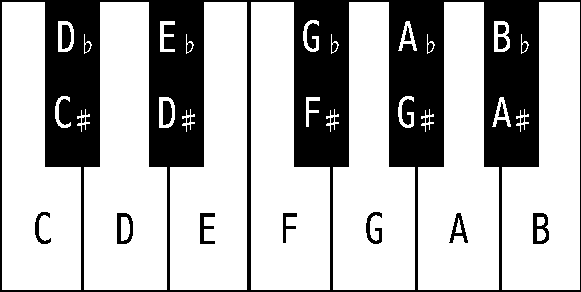
\includegraphics[width=0.9\textwidth]{res/pdf/4/scale/keys.pdf}
		\end{figure}
	\end{frame}
	
	\begin{frame}
		\frametitle{Section \ref{sec:interval} : 음정}
		\framesubtitle{음정들의 종류}
		아무튼, 간격이 달라지는 경우는 이 그림으로 설명이 가능합니다.
		\begin{figure}
			\centering
			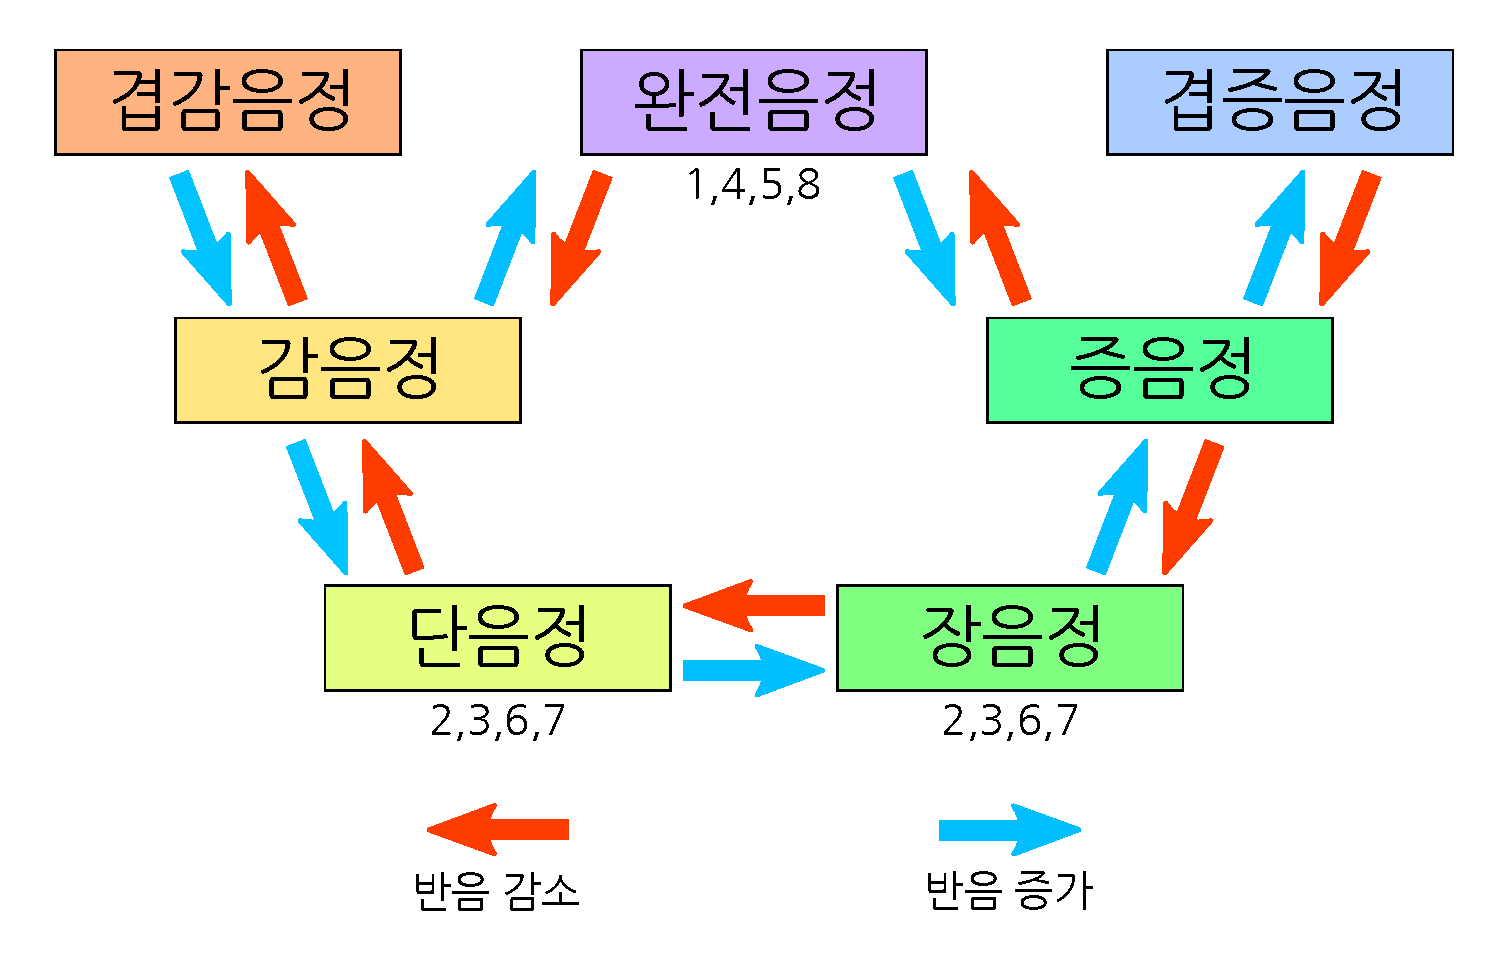
\includegraphics[width=\textwidth]{res/pdf/6/interval/relationship.pdf}
		\end{figure}
	\end{frame}
	
	\begin{frame}
		\frametitle{Section \ref{sec:interval} : 음정}
		\framesubtitle{......저게 뭔가요?}
		다음 표를 통해서 설명하겠습니다. 음계는 일반적인 도레미파솔라시도, 유식하게 말하자면 {\it 장음계} 기준입니다.
		\begin{table}[]
			\centering
			\small
			\begin{tabular}{|c|c|c|}
				\hline
				음정 & Quality & 특징 \\ \hline
				완전음정 & Perfect & 일반적인 1도, 4도, 5도, 8도.\\ \hline
				장음정 & Major & 일반적인 2도, 3도, 6도, 7도.\\ \hline
				단음정 & Minor & 장음정에서 간격이 반음 준 경우.\\ \hline
				증음정 & Augmented & 완전음정/장음정에서 간격이 반음 는 경우. \\ \hline
				감음정 & Diminished & 완전음정/단음정에서 간격이 반음 준 경우. \\ \hline
			\end{tabular}
		\end{table}
		겹감음정, 겹증음정은 말 그대로입니다.
	\end{frame}
	
	\begin{frame}
		\frametitle{Section \ref{sec:interval} : 음정}
		\framesubtitle{실습!}
		이런 건 실습을 통해서 늡니다. 한 번 음정을 구해보세요.\\
		\centering{\color{cyan} \href{run:res/mp3/6/test/q1.mp3}{실습 1.1}~~~~\href{run:res/mp3/6/test/q2.mp3}{실습 1.2}}
		\vskip -1pc
		\begin{figure}
			\centering
			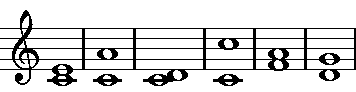
\includegraphics[width=\textwidth]{res/pdf/6/test/q1.pdf}
		\end{figure}
		\vskip -1.5pc
		\begin{figure}
			\centering
			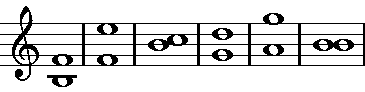
\includegraphics[width=\textwidth]{res/pdf/6/test/q2.pdf}
		\end{figure}
	\end{frame}
	
	\begin{frame}
		\frametitle{Section \ref{sec:interval} : 음정}
		\framesubtitle{풀이의 일부}
		각 줄별로 처음과 마지막에 있는 화음에 대해서만 풀이하겠습니다.
		\begin{itemize}
			\item 1. C-E\\
			간격이 3도이기에, 기준은 사이에 반음이 0쌍 있는 장3도가 됩니다. C-E 사이에 반음이 없기에 본 화음은 {\bf 장3도}입니다.
			\item 2. D-G\\
			간격이 4도이기에, 기준은 사이에 반음이 1쌍 있는 완전4도가 됩니다. D-G 사이에 반음이 한 쌍 있기에(E-F) 본 화음은 {\bf 완전4도}입니다.
		\end{itemize}
	\end{frame}
	
	\begin{frame}
		\frametitle{Section \ref{sec:interval} : 음정}
		\framesubtitle{풀이의 일부}
		\begin{itemize}
			\item 3. B-F\\
			간격이 5도이기에, 기준은 사이에 반음이 1쌍 있는 완전5도가 됩니다. B-F 사이에 반음이 두 쌍 있기에(B-C, E-F) 본 화음은 {\bf 감5도}입니다. 반음의 쌍이 많아지면 음의 간격이 줄어들기 때문입니다.
			\item 4. B-B\\
			간격이 1도이기에, 기준은 사이에 반음이 0쌍 있는 완전4도가 됩니다. B-B  사이에 반음이 없기에 본 화음은 {\bf 완전1도}입니다.
		\end{itemize}
	\end{frame}
	
	\begin{frame}
		\frametitle{Section \ref{sec:interval} : 음정}
		\framesubtitle{이게 끝인가요?}
		안타깝게도 그렇지 못합니다. 임시표를 아직 고려하지 않았기 때문입니다. 임시표를 고려하면 더 경우가 복잡해지는 경우가 많습니다. 다음이 {\color{cyan}\href{run:res/mp3/6/interval/etc.mp3}{그 예시들}}입니다.
		\begin{figure}
			\centering
			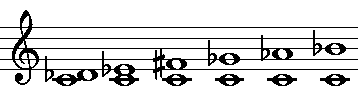
\includegraphics[width=\textwidth]{res/pdf/6/interval/etc.pdf}
		\end{figure}
	\end{frame}
	
	\subsection{Examples of intervals - Accidentals}
	\begin{frame}
		\frametitle{Section \ref{sec:interval} : 음정}
		\framesubtitle{임시표가 있다면......}
		다시 보겠습니다.
		\begin{figure}
			\centering
			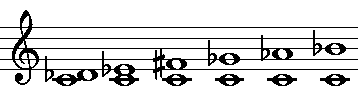
\includegraphics[width=0.6\textwidth]{res/pdf/6/interval/etc.pdf}
		\end{figure}
		도를 따질 때는 {\bf 임시표를 무시하고 따지면 됩니다.} 즉 저 경우에는 각각 2도, 3도, 4도, 5도, 6도, 7도가 되는 셈입니다.
	\end{frame}
	
	\begin{frame}
		\frametitle{Section \ref{sec:interval} : 음정}
		\framesubtitle{임시표가 있다면......}
		임시표가 없었으면 음정들은 각각 장2도, 장3도, 완전4도, 완전5도, 장6도, 장7도였겠죠.
		\begin{figure}
			\centering
			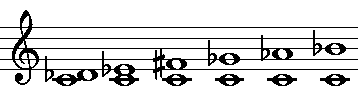
\includegraphics[width=0.6\textwidth]{res/pdf/6/interval/etc.pdf}
		\end{figure}
		하지만 음정 간의 관계를 이용하면 이는 각각 단2도, 단3도, 증4도, 감5도, 단6도, 단7도라는 것을 알 수 있습니다. 재미있는 사실은 증4도와 감5도가 실제로는 같은 음정이라는 것입니다.
	\end{frame}
	
	\begin{frame}
		\frametitle{Section \ref{sec:interval} : 음정}
		\framesubtitle{실습!}
		한 번 더 실습을 하겠습니다. 이번에는 임시표들이 즐비하네요.
		\centering{\color{cyan} \href{run:res/mp3/6/test/q3.mp3}{실습 2.1}~~~~\href{run:res/mp3/6/test/q4.mp3}{실습 2.2}}
		\vskip -1pc
		\begin{figure}
			\centering
			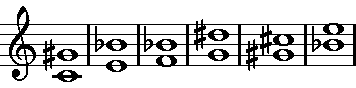
\includegraphics[width=\textwidth]{res/pdf/6/test/q3.pdf}
		\end{figure}
		\vskip -1.5pc
		\begin{figure}
			\centering
			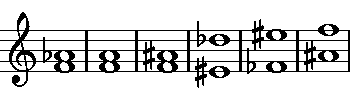
\includegraphics[width=\textwidth]{res/pdf/6/test/q4.pdf}
		\end{figure}
	\end{frame}
	
	\begin{frame}
		\frametitle{Section \ref{sec:interval} : 음정}
		\framesubtitle{풀이의 일부}
		\begin{itemize}
			\item 5. C-G$\sharp$\\
			간격이 5도이기에, 기준은 사이에 반음이 1쌍 있는 장3도가 됩니다. C-G$\sharp$ 사이에 반음이 1쌍 있고 올림표를 통해 간격이 반음 증가했기에 본 화음은 {\bf 증5도}입니다.
			\item 6. B$\flat$-E\\
			간격이 4도이기에, 기준은 사이에 반음이 1쌍 있는 완전4도가 됩니다. B$\flat$-E 사이에 반음이 1쌍 있고 내림표를 통해 간격이 반음 증가했기에 본 화음은 {\bf 증4도}입니다.
		\end{itemize}
	\end{frame}
	
	\begin{frame}
		\frametitle{Section \ref{sec:interval} : 음정}
		\framesubtitle{풀이의 일부}
		\begin{itemize}
			\item 7. F-A$\flat$\\
			간격이 3도이기에, 기준은 사이에 반음이 0쌍 있는 장3도가 됩니다. C-G$\sharp$ 사이에 반음이 없고 내림표를 통해 간격이 반음 감소했기에 본 화음은 {\bf 단3도}입니다.
			\item 8. A$\sharp$-F\\
			간격이 6도이기에, 기준은 사이에 반음이 1쌍 있는 장6도가 됩니다. A$\sharp$-F 사이에 반음이 1쌍 있고 올림표를 통해 간격이 반음 감소했기에 본 화음은 {\bf 단6도}입니다.
		\end{itemize}
	\end{frame}
	
	\begin{frame}
		\frametitle{Section \ref{sec:interval} : 음정}
		\framesubtitle{음정을 마치며......}
		음정의 개념을 잘 이해하셨나요? 이러한 개념을 처음 접하신 분들에게는 쉽지 않았을 것으로 생각됩니다. 그래도 머릿속에 음정들의 관계도를 집어넣으면 이해가 쉽지 않을까 추측합니다. 그럼 이제 이 음정의 기본 지식들을 가지고 음계를 이야기하도록 하겠습니다.
	\end{frame}
	
	\section{Section 7 : Scale}\label{sec:scale}
	\subsection{Definition of scale}
	\begin{frame}
		\frametitle{Section \ref{sec:scale} : 음계}
		\framesubtitle{음계의 정의}
		\begin{definition}[음계, 音階, Scale]
			\begin{itemize}
				\item 일정한 음정의 순서로 음을 차례로 늘어놓은 것. 동양 음악은 5음 음계, 서양 음악은 7음 음계를 기초로 한다. - 표준국어대사전
			\end{itemize}
		\end{definition}
	\end{frame}
	
	\begin{frame}
		\frametitle{Section \ref{sec:scale} : 음계}
		\framesubtitle{음계의 정의}
		중학교 때 단소를 열심히 부셨던 분들은 `중임무황태'가 기억나실지도 모릅니다. 음이름으로 하자면 `사가다라마(GACDE)'이죠. 이것도 음계입니다. 결국 음계라는 것은 서로 구분되는 음들을 모아 놓은 것이며, 시대와 문화에 따라 다양한 양상을 보여왔습니다. 
	\end{frame}
	
	\subsection{Chromatic scale}
	\begin{frame}
		\frametitle{Section \ref{sec:scale} : 음계}
		\framesubtitle{반음계(chromatic scale)}
		현대 음악에서 기본이 되는 음계는 바로 {\bf 반음계(chromatic scale)}입니다. 12개의 반음으로 구분되어 있으며, 각 간격이 정확히 반음입니다. {\color{cyan}\href{run:res/mp3/7/scale/chromatic_ascend.mp3}{상행}}과 {\color{cyan}\href{run:res/mp3/7/scale/chromatic_descend.mp3}{하행}}을 각각 들어보세요.
		\begin{figure}
			\centering
			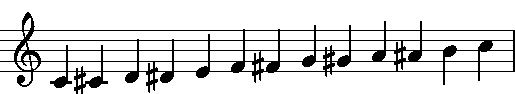
\includegraphics[width=\textwidth]{res/pdf/7/scale/chromatic_ascend.pdf}
		\end{figure}
		\vskip -1.5pc
		\begin{figure}
			\centering
			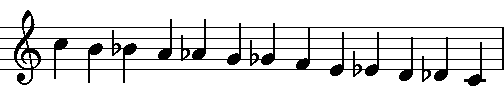
\includegraphics[width=\textwidth]{res/pdf/7/scale/chromatic_descend.pdf}
		\end{figure}
	\end{frame}
	
	\begin{frame}
		\frametitle{Section \ref{sec:scale} : 음계}
		\framesubtitle{반음계(chromatic scale)}
		반음계에서 각 음들의 관계는 다음과 같이 12등분된 원으로 나타낼 수 있습니다. 이 음들만으로 (요즘은) 모든 것을 만들어내기 때문에, 어떤 음이 어떤 음인지 아셨으면 좋겠습니다.
		\begin{figure}
			\centering
			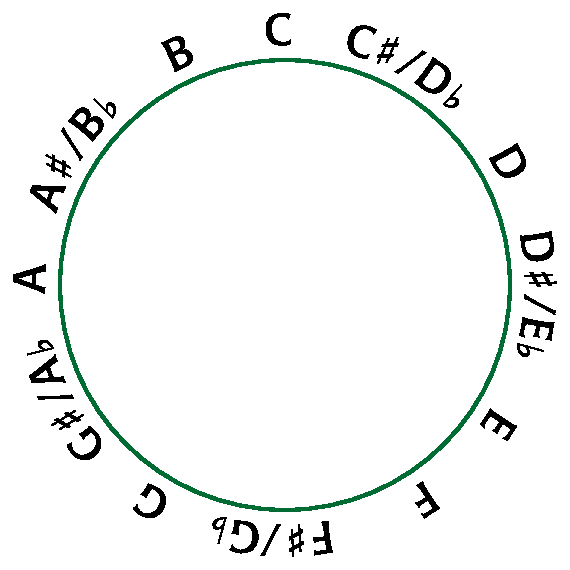
\includegraphics[width=0.5\textwidth]{res/pdf/7/scale/pitch_circle.pdf}
		\end{figure}
	\end{frame}
	
	\subsection{Diatonic scale}
	\begin{frame}
		\frametitle{Section \ref{sec:scale} : 음계}
		\framesubtitle{온음계(diatonic scale)}
		반음계는 모든 음들을 다 포함하고 있지만, 음의 기본 간격이 `온음'이라는 사실은 기억하셔야 합니다. 때문에 온음이 주된 간격이 되는 음계들이 필요해졌습니다. 이런 음계들을 {\bf 온음계(diatonic scale)}이라고 합니다.
	\end{frame}
	
	\begin{frame}
		\frametitle{Section \ref{sec:scale} : 음계}
		\framesubtitle{온음계(diatonic scale)}
		얼핏 생각해보면 모든 음의 간격을 온음으로 하는 것이 합리적으로 생각될 수 있습니다. 실제로 그런 음계도 있고요(whole tone scale). 그런 `6음계'($ 12/2=6 $)나 5음계(중임무황태)도 여러 문화에서 발견되어왔습니다만, 일단은 현대 음악의 {\bf 7음계}를 따라가겠습니다.
	\end{frame}
	
	\subsection{Major scale}
	\begin{frame}
		\frametitle{Section \ref{sec:scale} : 음계}
		\framesubtitle{장음계(major scale)}
		사실 우리는 이미 앞에서 온음계 하나를 가지고 공부를 해봤습니다. 바로 {\bf 장음계}입니다.
		\begin{figure}[!h]
			\centering
			{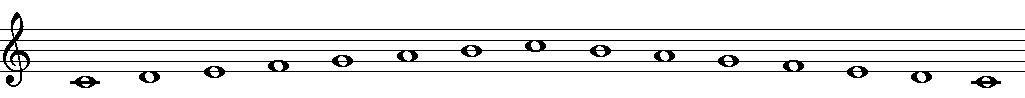
\includegraphics[width=\textwidth]{res/pdf/4/syllable/doremi.pdf}}
		\end{figure}
		\ref{sec:notations}장에서 본 것 같지 않나요? 흔히 {\bf `도레미파솔라시도'}라고 음을 붙이는 익숙한 `음계'이죠.
	\end{frame}
	
	\begin{frame}
		\frametitle{Section \ref{sec:scale} : 음계}
		\framesubtitle{장음계(major scale)}
		이 무의식적으로 당연하다 여겼던 {\color{cyan}\href{run:res/mp3/7/scale/major_ascend.mp3}{장음계}}를 살펴봅시다. 
		\begin{figure}[!h]
			\centering
			{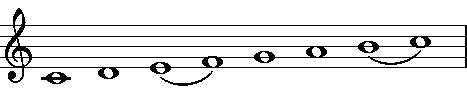
\includegraphics[width=\textwidth]{res/pdf/7/scale/major_ascend.pdf}}
		\end{figure}
		12개의 반음 사이에 7개의 음을 넣으니 반음 관계가 2개가 생성되며, 이는 3-4, 7-8에 생성됩니다. 이음줄은 두 음이 반음 간격이라는 것을 의미합니다.
	\end{frame}
	
	\begin{frame}
		\frametitle{Section \ref{sec:scale} : 음계}
		\framesubtitle{장음계(major scale)}
		이러한 장음계는 대체로 밝은 분위기를 내며, 이를 계승하는 화음들이나 곡들도 그러한 분위기를 내는 경우가 많습니다. `장조'랑 밀접한 관련을 가지고 있죠.
	\end{frame}
	
	\subsection{Minor scale}
	\begin{frame}
		\frametitle{Section \ref{sec:scale} : 음계}
		\framesubtitle{단음계(minor scale)}
		또 다른 유명한 온음계로는 단음계(minor scale)가 있습니다. 장음계와는 여러 가지로 대조가 되는 음계입니다. 단음계는 보통 3종류로 나눕니다. 각각 {\bf `자연 단음계', `화음 단음계', `가락 단음계'}입니다.
	\end{frame}
	
	\begin{frame}
		\frametitle{Section \ref{sec:scale} : 음계}
		\framesubtitle{자연 단음계(natural minor scale)}
		우선 기본이 되는 자연 단음계입니다.
		\begin{figure}[!h]
			\centering
			{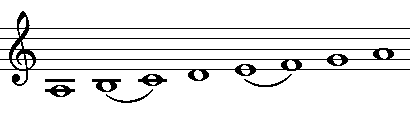
\includegraphics[width=\textwidth]{res/pdf/7/scale/natural_minor_ascend.pdf}}
		\end{figure}
		장음계와 차이점은 우선 시작하는(나중에 {\it 으뜸음}이라 할) 음이 {\bf `라'}라는 것이며, 반음는 2-3, 5-6에 생성됩니다.
	\end{frame}
	
	\begin{frame}
		\frametitle{Section \ref{sec:scale} : 음계}
		\framesubtitle{자연 단음계(natural minor scale)}
		상행 하행을 모두 보자면 {\color{cyan}\href{run:res/mp3/7/scale/natural_minor.mp3}{다음과 같습니다}}.
		\begin{figure}[!h]
			\centering
			{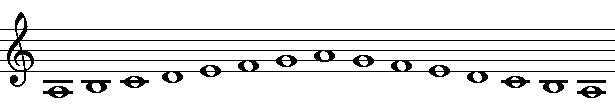
\includegraphics[width=\textwidth]{res/pdf/7/scale/natural_minor.pdf}}
		\end{figure}
		다만 이 음계는 제7도와 제8도의 간격이 온음이여서, 진행이나 화음이 부자연스러운 경향이 있습니다. 나중에 배우겠지만 제7도는 제8도(제1도)로 가려는 경향성이 크기 때문입니다.
	\end{frame}
	
	\begin{frame}
		\frametitle{Section \ref{sec:scale} : 음계}
		\framesubtitle{화성 단음계(harmonic minor scale)}
		그럼 {\color{cyan}\href{run:res/mp3/7/scale/harmonic_minor.mp3}{화성 단음계}}는 무엇인고 하니, 간격 문제를 해결하기 위해 자연 단음계에서 제7음을 반음 올린 음계입니다.
		\begin{figure}[!h]
			\centering
			{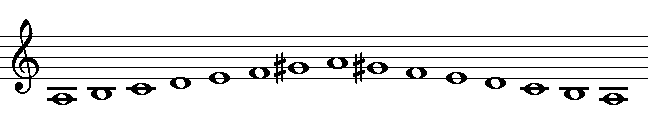
\includegraphics[width=\textwidth]{res/pdf/7/scale/harmonic_minor.pdf}}
		\end{figure}
		그런데 이러면 제6도와 제7도의 간격이 {\bf 증2도}가 되기에, 멜로디를 진행할 때는 알맞지 않죠. 
	\end{frame}
	
	\begin{frame}
		\frametitle{Section \ref{sec:scale} : 음계}
		\framesubtitle{가락 단음계(melodic minor scale)}
		이를 해결하기 위해, 제6도도 반음을 올린 음계가 {\color{cyan}\href{run:res/mp3/7/scale/melodic_minor.mp3}{가락 단음계}}입니다. 그러면 모든 간격이 장2도와 단2도로 구성되기 때문입니다.
		\begin{figure}[!h]
			\centering
			{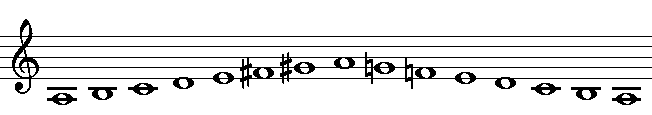
\includegraphics[width=\textwidth]{res/pdf/7/scale/melodic_minor.pdf}}
		\end{figure}
		다만 음을 내려갈 때는 자연 단음계와 똑같이 진행됩니다.
	\end{frame}
	
	\begin{frame}
		\frametitle{Section \ref{sec:scale} : 음계}
		\framesubtitle{그래서 뭘 쓰라는 건가요.}
		일단 장음계의 경우도 화성/가락 장음계가 있으나, 대개 자연 장음계를 많이 씁니다. 조화로우니까요. 다만 제가 보기에 완벽한 단음계는 없습니다. 하지만 이 세 단음계는 서로를 보완해줄 수 있습니다. 변형해서 쓰는 경우도 많고요. 이런 음계의 개념을 이해하신다면 곧 다룰 `조와 조성'을 잘 이해할 수 있을 겁니다.  
	\end{frame}
	
	\section{Section 8 : Tonality}\label{sec:tonality}
	\subsection{Definition of tonality}
	\begin{frame}
		\frametitle{Section \ref{sec:tonality} : 조성}
		\framesubtitle{조성의 정의}
		\begin{definition}[조성, 調性, Tonality]
			\begin{itemize}
				\item 주음(主音) 및 그 화음에 따라 결정되는 곡조의 성질. - 표준국어대사전
			\end{itemize}
		\end{definition}
	\end{frame}
	
	\begin{frame}
		\frametitle{Section \ref{sec:tonality} : 조성}
		\framesubtitle{조성의 정의}
		직관적으로 설명하자면, 조성은 기본적으로 음악의 {\bf `주된 음, 또는 화음'}을 의미한다고 볼 수 있습니다. 대부분의 현대 음악은 주된 음이 있고, 이에 따라 2순위, 3순위로 주된 음들이 나타나기 때문이죠.
	\end{frame}
	
	\begin{frame}
		\frametitle{Section \ref{sec:tonality} : 조성}
		\framesubtitle{음의 역할}
		7음계의 각 음에는 역할 내지는 이름이 붙어 있습니다.
		\begin{table}[!h]
			\centering
			\begin{tabular}{|c|c|c|}
				\hline
				도 & 음의 이름 & Scale degree \\ \hline
				제1음 & 으뜸음 & Tonic \\ \hline
				제2음 & 위으뜸음 & Supertonic \\ \hline
				제3음 & 가온음 & Mediant \\ \hline
				제4음 & 버금딸림음 & Subdominant \\ \hline
				제5음 & 딸림음 & Dominant \\ \hline
				제6음 & 버금가온음 & Submediant \\ \hline
				제7음 & 이끔음 & Leading tone / Subtonic \\ \hline
				제8음 & 으뜸음 & Tonic(octave) \\ \hline
			\end{tabular}
		\end{table}
	\end{frame}
	
	\begin{frame}
		\frametitle{Section \ref{sec:tonality} : 조성}
		\framesubtitle{음의 역할}
		그중에서도 {\bf 으뜸음}과 {\bf 딸림음}, {\bf 버금딸림음}은 들어보셨을 법 합니다. 각각 제1도, 제5도, 제4도입니다. 이 세 음들은 조성에서 매우 중요한 역할을 하는 음들입니다. 애초에 완전음정이기도 하고요. 그 중 이끔음은 {\bf 조를 대표하는 음입니다}. 이 음의 음이름을 따서 음악의 조를 정하는 것이죠.
	\end{frame}
	
	\subsection{Major and Minor}
	\begin{frame}
		\frametitle{Section \ref{sec:tonality} : 조성}
		\framesubtitle{음의 역할}
		우선 장조와 단조를 정의하고 가야겠군요. 조성을 지금 배우는 이유는 매우 간단합니다. 음계로 정의가 가능하기 때문이죠. {\bf 장음계를 기본으로 하면 장조, 단음계를 기본으로 하면 단조입니다.} 단조의 경우 자연단음계를 기준으로 합니다.
	\end{frame}
	
	\begin{frame}
		\frametitle{Section \ref{sec:tonality} : 조성}
		\framesubtitle{장조}
		예시를 들어볼까요? 으뜸음을 마로 하고, 장조로 음계를 만들어봅시다. 그러면 {\bf `마'가 으뜸음이 되도록 장음계를 만들면} 끝입니다. 장음계는 3-4, 7-8이 반음 간격이었죠. 그러면 다음과 같이 되겠네요.
		\begin{figure}
			\centering
			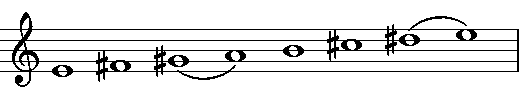
\includegraphics[width=\textwidth]{res/pdf/8/scale/major/E_major.pdf}
		\end{figure}
		\vskip -1.5pc
		이게 마장조의 음계입니다! 임시표를 무시하고 각기 다른 음들이 나와야 한다는 사실에 유념하세요.
	\end{frame}
	
	\begin{frame}
		\frametitle{Section \ref{sec:tonality} : 조성}
		\framesubtitle{실습!}
		자, 그러면 준비 되셨나요? 음은 총 12개가 있습니다. 각 음들을 기준으로 12개의 장음계를 직접 다 그려보세요. 네? 어떤 음들은 플랫과 샤프을 사용하면 2개가 나온다고요? 글쎄요......직접 종이에 해 보세요. $\sharp$과 $\flat$을  붙여가면서요.
		\begin{figure}
			\centering
			\includegraphics[width=\textwidth]{res/pdf/8/blank.pdf}
		\end{figure}
	\end{frame}
	
	\begin{frame}
		\frametitle{Section \ref{sec:tonality} : 조성}
		\framesubtitle{실습의 정답}
		이번에는 특별히 정답을 지금 공개하겠습니다.\\
		\begin{figure} \color{cyan}{\href{run:res/mp3/8/scale/major/C_major.mp3}{다장조}}
			{\centering \includegraphics[width=\textwidth]{res/pdf/8/scale/major/C_major.pdf}}
		\end{figure}
		\vskip -2pc
		\begin{figure} \color{cyan}{\href{run:res/mp3/8/scale/major/F_major.mp3}{바장조}}
			{\centering \includegraphics[width=\textwidth]{res/pdf/8/scale/major/F_major.pdf}}
		\end{figure}
	\end{frame}
	
	\begin{frame}
		\frametitle{Section \ref{sec:tonality} : 조성}
		\framesubtitle{실습의 정답}
		\begin{figure} \color{cyan}{\href{run:res/mp3/8/scale/major/B_flat_major.mp3}{내림나장조}}
			{\centering \includegraphics[width=\textwidth]{res/pdf/8/scale/major/B_flat_major.pdf}}
		\end{figure}
		\vskip -2pc
		\begin{figure} \color{cyan}{\href{run:res/mp3/8/scale/major/E_flat_major.mp3}{내림마장조}}
			{\centering \includegraphics[width=\textwidth]{res/pdf/8/scale/major/E_flat_major.pdf}}
		\end{figure}
	\end{frame}
	
	\begin{frame}
		\frametitle{Section \ref{sec:tonality} : 조성}
		\framesubtitle{실습의 정답}
		\begin{figure} \color{cyan}{\href{run:res/mp3/8/scale/major/A_flat_major.mp3}{내림가장조}}
			{\centering \includegraphics[width=\textwidth]{res/pdf/8/scale/major/A_flat_major.pdf}}
		\end{figure}
		\vskip -2pc
		\begin{figure} \color{cyan}{\href{run:res/mp3/8/scale/major/D_flat_major.mp3}{내림라장조}}
			{\centering \includegraphics[width=\textwidth]{res/pdf/8/scale/major/D_flat_major.pdf}}
		\end{figure}
	\end{frame}
	
	\begin{frame}
		\frametitle{Section \ref{sec:tonality} : 조성}
		\framesubtitle{실습의 정답}
		\begin{figure} \color{cyan}{\href{run:res/mp3/8/scale/major/G_flat_major.mp3}{내림사장조}}
			{\centering \includegraphics[width=\textwidth]{res/pdf/8/scale/major/G_flat_major.pdf}}
		\end{figure}
		\vskip -2pc
		\begin{figure} \color{cyan}{\href{run:res/mp3/8/scale/major/B_major.mp3}{나장조}}
			{\centering \includegraphics[width=\textwidth]{res/pdf/8/scale/major/B_major.pdf}}
		\end{figure}
	\end{frame}
	
	\begin{frame}
		\frametitle{Section \ref{sec:tonality} : 조성}
		\framesubtitle{실습의 정답}
		\begin{figure} \color{cyan}{\href{run:res/mp3/8/scale/major/E_major.mp3}{마장조}}
			{\centering \includegraphics[width=\textwidth]{res/pdf/8/scale/major/E_major.pdf}}
		\end{figure}
		\vskip -2pc
		\begin{figure} \color{cyan}{\href{run:res/mp3/8/scale/major/A_major.mp3}{가장조}}
			{\centering \includegraphics[width=\textwidth]{res/pdf/8/scale/major/A_major.pdf}}
		\end{figure}
	\end{frame}
	
	\begin{frame}
		\frametitle{Section \ref{sec:tonality} : 조성}
		\framesubtitle{실습의 정답}
		\begin{figure} \color{cyan}{\href{run:res/mp3/8/scale/major/D_major.mp3}{라장조}}
			{\centering \includegraphics[width=\textwidth]{res/pdf/8/scale/major/D_major.pdf}}
		\end{figure}
		\vskip -2pc
		\begin{figure} \color{cyan}{\href{run:res/mp3/8/scale/major/G_major.mp3}{사장조}}
			{\centering \includegraphics[width=\textwidth]{res/pdf/8/scale/major/G_major.pdf}}
		\end{figure}
	\end{frame}
	
	\begin{frame}
		\frametitle{Section \ref{sec:tonality} : 조성}
		\framesubtitle{임시표를 보아하니......}
		배열에서 눈치채셨나요? 처음에는 $\flat$을 쓰다가 다시 $\sharp$으로 넘어오며, 임시표가 붙는 순서가 있다는 것을요.\\
		$\flat$은 시미라레솔도파로(그냥 계이름으로 부르겠습니다) 붙입니다. 반면에  $\sharp$은 파도솔레라미시 순서대로 붙습니다. 순서가 반대죠. 영어권에서는 {\bf B}etter {\bf E}at {\bf A} {\bf D}oughnut {\bf G}et {\bf C}offee {\bf F}irst로 외운다고 하더군요. 이 순서대로 {\bf 조표}를 붙이면 됩니다. 그러면 바로 임시표 없이 도레미파솔라시도로 이름을 매길 수 있으니까요.
	\end{frame}
	
	\subsection{Circle of fifth}
	\begin{frame}
		\frametitle{Section \ref{sec:tonality} : 조성}
		\framesubtitle{5도권(Circle of fifth)}
		이를 그림으로 나타내면 다음과 같습니다.
		\begin{figure}
			\centering
			\includegraphics[height=0.7\textheight]{res/pdf/8/circle_of_fifth.pdf}
		\end{figure}
	\end{frame}
	%Microsoft Powerpoint -> Export to .emf -> Inkscape -> Export to .pdf after altering the circles' stroke width to 0px. Quite complicated.
	
	\begin{frame}
		\frametitle{Section \ref{sec:tonality} : 조성}
		\framesubtitle{5도권(Circle of fifth)}
		이를 5도권이라 합니다. 그 이유는 {\bf 완전5도씩 올라가거나 내려가면 이러한 순환이 만들어지기 때문입니다.} 참 신기하죠. 이 순환이 조표의 순서와 정확히 일치한다는 사실이 말입니다. 찬찬히 음미해보시길 바랍니다.\\
		여기서 설명은 생략하지만 단조의 경우에도 성립합니다. 으뜸음을 `라'로 잡은 다음에 한 번 해보세요.
	\end{frame}
	
	\begin{frame}
		\frametitle{Section \ref{sec:tonality} : 조성}
		\framesubtitle{5도권(Circle of fifth)}
		아무튼 5도권의 개념은 이렇게 간단하게 넘어가지만 추후에 다시 등장할 겁니다. 마지막으로 플랫과 샤프의 개수를 통해 곡의 조성을 알 수 있는 방법을 구하고 넘어가겠습니다.
	\end{frame}
	
	\begin{frame}
		\frametitle{Section \ref{sec:tonality} : 조성}
		\framesubtitle{플랫이 있는 경우.....}
		`시미라레솔도파'의 플랫의 경우를 보겠습니다.
		\begin{figure}
			\centering
			\includegraphics[width=\textwidth]{res/pdf/8/tone/flat.pdf}
		\end{figure}
		플랫의 경우 마지막으로 붙은 플랫에서 4도를 내려가면(즉 5도를 올라가면) 으뜸음이 나옵니다.
		\vskip -1.5pc
		\begin{table}
			\small
			\begin{tabular}{|c|c|c|c|c|c|c|c|}
				\hline
				순서 & B & E & A & D & G & C & F \\ \hline
				개수 & 1개 & 2개 & 3개 & 4개 & 5개 & 6개 & 7개 \\ \hline
				으뜸음 & 바 & 내림나 & 내림마 & 내림가 & 내림라 & 내림사 & 내림다 \\ \hline
				Tonic & F & B$\flat$ & E$\flat$ & A$\flat$ & D$\flat$ & G$\flat$ & C$\flat$ \\ \hline
			\end{tabular}
		\end{table}
	\end{frame}
	
	\begin{frame}
		\frametitle{Section \ref{sec:tonality} : 조성}
		\framesubtitle{샤프이 있는 경우......}
		`파도솔레라미시'의 샤프의 경우를 보겠습니다.
		\begin{figure}
			\centering
			\includegraphics[width=\textwidth]{res/pdf/8/tone/sharp.pdf}
		\end{figure}
		샤프의 경우 마지막으로 붙은 샤프에서 2도를 올라가면 으뜸음이 나옵니다.
		\vskip -0.5pc
		\begin{table}
			\small
			\begin{tabular}{|c|c|c|c|c|c|c|c|}
				\hline
				순서 & F & C & G & D & A & E & B \\ \hline
				개수 & 1개 & 2개 & 3개 & 4개 & 5개 & 6개 & 7개 \\ \hline
				으뜸음 & 사 & 라 & 가 & 마 & 나 & 올림바 & 올림다 \\ \hline
				Tonic & G & D & A & E & B & F$\sharp$ & C$\sharp$ \\ \hline
			\end{tabular}
		\end{table}
	\end{frame}
	
	\begin{frame}
		\frametitle{Section \ref{sec:tonality} : 조성}
		\framesubtitle{단조는요?}
		단조는 각 경우에 대해서 똑같이 한 다음에 3도 내려가면 됩니다.
		\begin{table}
			\small
			\begin{tabular}{|c|c|c|c|c|c|c|c|}
				\hline
				순서($\flat$) & B & E & A & D & G & C & F \\ \hline
				개수 & 1개 & 2개 & 3개 & 4개 & 5개 & 6개 & 7개 \\ \hline
				으뜸음 & 라 & 사 & 다 & 바 & 내림나 & 내림마 & 내림가 \\ \hline
				Tonic & d & g & c & f & b$\flat$ & g$\flat$ & a$\flat$ \\ \hline
			\end{tabular}
		\end{table}
		\begin{table}
			\small
			\begin{tabular}{|c|c|c|c|c|c|c|c|}
				\hline
				순서($\sharp$) & F & C & G & D & A & E & B \\ \hline
				개수 & 1개 & 2개 & 3개 & 4개 & 5개 & 6개 & 7개 \\ \hline
				으뜸음 & 마 & 나 & 올림바 & 올림다 & 올림사 & 올림라 & 올림가 \\ \hline
				Tonic & e & b & f$\sharp$ & c$\sharp$ & g$\sharp$ & d$\sharp$ & a$\sharp$ \\ \hline
			\end{tabular}
		\end{table}
	\end{frame}
	
	\begin{frame}
		\frametitle{Section \ref{sec:tonality} : 조성}
		\framesubtitle{조성을 마무리하며}
		조성은 결국 시작점이 다르기에 나타나는 현상입니다. 어떠한 음을 주된 음으로 놓을 것이냐가 분위기를 만들어나가는 것이죠. 장조와 단조 사이의 분위기 차이도 있지만, 으뜸음에 따라서도 분위기가 미세하게 차이가 납니다.\\
		달리 보자면, 조성을 파악하면 주된 화음이 무엇인지 알 수 있습니다. 이에 대해서는 이어서 설명하도록 하겠습니다. 
	\end{frame}
	
	\section{Section 9 : Chord}\label{sec:chord}
	\subsection{Definition of chord}
	\begin{frame}
		\frametitle{Section \ref{sec:chord} : 화음}
		\framesubtitle{화음의 정의}
		드디어 코드, 달리 말하면 화음의 설명을 시작할 수 있겠군요.
		\begin{definition}[화음, 和音, Chord]
			{\bf 높이가 다른 둘 이상의 음이 함께 울릴 때 어울리는 소리.} -표준국어대사전
		\end{definition}
		다만 음이 3개 이상일 때만 화음이라고 정의하기도 하나 봅니다. 실제로 화음에 음이 최소 3개는 있어야 콕 집어서 분류도 할 수 있고요.
	\end{frame}
	
	\begin{frame}
		\frametitle{Section \ref{sec:chord} : 화음}
		\framesubtitle{화음과 관련된 이야기들}
		화음은 기본적으로 `기본음'이라 불리는, 하나의 음을 기본으로 형성됩니다. 이 기본음은 기본적으로는, 화음의 가장 낮은 음입니다. 여기에 추가적으로 붙는 음들이 그 화음의 성질을 결정하는 것이고요. 일단 종종 쓰이는 화음 몇 개를 음정을 통해 정의하면서 시작하겠습니다.\\
		%그리고 보통 `코드'라는 말을 ``이거 반주 코드가 Dm7이잖아''라는 식으로 주로 쓰는데, 그런 용례가 틀리지는 않지만 {\bf 코드가 화음을 뜻한다는 것은 알아 두세요.}
	\end{frame}
	
	\subsection{Definition of triad}
	\begin{frame}
		\frametitle{Section \ref{sec:chord} : 화음}
		\framesubtitle{3화음(Triad)}
		보통 화음을 만들 때는 {\bf 3도씩 쌓아서 만듭니다.} 왜냐고요? 그러면 안정하게 들리거든요. 2도나 4도씩 쌓아서 올리는 것보다요. 저 기본적인 사실을 꼭 기억하시기 바랍니다.
	\end{frame}
	
	\begin{frame}
		\frametitle{Section \ref{sec:chord} : 화음}
		\framesubtitle{3화음(Triad)}
		즉 1도, 3도, 5도를 쌓아올림으로써, 우리는 3화음이라 불리는 화음을 만들 수  있습니다. 그런데 3도나 5도나 음정의 관점으로 보자면 여러 가지가 있잖아요? 그래서 기본이 되는 화음이 4종류가 나옵니다. 바로 장3화음, 단3화음, 증3화음, 감3화음입니다.
	\end{frame}
	
	\begin{frame}
		\frametitle{Section \ref{sec:chord} : 화음}
		\framesubtitle{3화음(Triad)}
		이들을 분석하자면 다음과 같습니다.
		\begin{table}
			\begin{tabular}{|c|c|c|c|}
				\hline
				& 3도 & 5도 & 기본음이 C일 때 표기법 \\ \hline
				\color{cyan}\href{run:res/mp3/9/chord/triad/C_major.mp3}{장3화음} & 장3도 & 완전5도 & {\bf C}, CM, Cmaj, Cma, C$\Delta$\\ \hline
				\color{cyan}\href{run:res/mp3/9/chord/triad/C_minor.mp3}{단3화음} & 단3도 & 완전5도 & {\bf Cm}, C-, Cmi, Cmin\\ \hline
				\color{cyan}\href{run:res/mp3/9/chord/triad/C_aug.mp3}{증3화음} & 장3도 & 증5도 & {\bf Caug}, C+, C$^+$\\ \hline
				\color{cyan}\href{run:res/mp3/9/chord/triad/C_dim.mp3}{감3화음} & 단3도 & 감5도 & {\bf Cdim}, C$\degree$\\ \hline
			\end{tabular}
		\end{table}
		\vskip -1.5pc
		\begin{figure}
			\centering
			\includegraphics[width=\textwidth]{res/pdf/9/chord/triad.pdf}
		\end{figure}
	\end{frame}
	
	\begin{frame}
		\frametitle{Section \ref{sec:chord} : 화음}
		\framesubtitle{3화음(Triad)}
		각 음들을 기본음으로 하는 3화음들을 들어보세요.
		\begin{figure}
			\centering
			\color{cyan}\href{run:res/mp3/9/scale/chromatic_major_chord.mp3}{장3화음(Major triad)}
			\includegraphics[width=\textwidth]{res/pdf/9/scale/major.pdf}
		\end{figure}
		\begin{figure}
			\centering
			\color{cyan}\href{run:res/mp3/9/scale/chromatic_minor_chord.mp3}{단3화음(Minor triad)}
			\includegraphics[width=\textwidth]{res/pdf/9/scale/minor.pdf}
		\end{figure}
	\end{frame}
	
	\begin{frame}
		\frametitle{Section \ref{sec:chord} : 화음}
		\framesubtitle{3화음(Triad)}
		\begin{figure}
			\centering
			\color{cyan}\href{run:res/mp3/9/scale/chromatic_augmented_chord.mp3}{증3화음(Augmented triad)}
			\includegraphics[width=\textwidth]{res/pdf/9/scale/augmented.pdf}
		\end{figure}
		\begin{figure}
			\centering
			\color{cyan}\href{run:res/mp3/9/scale/chromatic_diminished_chord.mp3}{감3화음(Diminished triad)}
			\includegraphics[width=\textwidth]{res/pdf/9/scale/diminished.pdf}
		\end{figure}
	\end{frame}
	
	\begin{frame}
		\frametitle{Section \ref{sec:chord} : 화음}
		\framesubtitle{3화음(Triad)}
		이 중 장3화음과 단3화음은 협화음(어울림화음)입니다. 다음 장에서 배울 `다이어토닉 코드'에서도 단골로 등장할 화음들이기 때문입니다. 다만 증3화음과 감3화음은 안정적이지는 않습니다. 물론 적절하게 진행 도중에 사용하면, 새로운 분위기를 낼 수도 있습니다. 
	\end{frame}
	
	\subsection{Definition of 7th chord}
	\begin{frame}
		\frametitle{Section \ref{sec:chord} : 화음}
		\framesubtitle{7화음(7th chord)}
		이 3화음에 7음을 쌓아 올린 것이 7화음입니다. 음이 4개가 있어서 `4화음'이라고도 합니다. 다만 조금 엄격하게 말하자면, 저 `4화음'이라는 표현은 틀린 표현입니다. 원래는 3화음도 `5화음'이라고 말해야 옳습니다. 왜냐하면 3화음의 `3'은 성부의 숫자거든요. 때문에 다음과 같은 동치관계가 나타납니다.
		\begin{itemize}
			\item 5화음 = 3성화음
			\item 7화음 = 4성화음
		\end{itemize}
		......하지만 그냥 통상적으로 3화음/7화음이라고 많이 말하기에(영칭부터 Triad, Seventh이니까요), 이해만 잘 하시면 됩니다.
	\end{frame}
	
	\begin{frame}
		\frametitle{Section \ref{sec:chord} : 화음}
		\framesubtitle{7화음(7th chord)}
		많은 사람들의 생각과는 달리 7화음은 {\bf 불협화음}입니다. 불협이라고 해서 쓰지 말라는 것이 아니라, 안정된 화음이 아니라는 것입니다.
		기본적인 이유는 7음이랑 1음이랑 간격이 상당히 가까워서지만, 이는 7화음의 종류에 따라 달라집니다.
	\end{frame}
	
	\begin{frame}
		\frametitle{Section \ref{sec:chord} : 화음}
		\framesubtitle{7화음(7th chord)}
		여백의 문제로 4개만 다루자면 다음과 같습니다.
		\begin{table}
			\begin{tabular}{|c|c|c|c|c|}
				\hline
				& 3도 & 5도 & 7도 & 기본음이 C일 때 표기법 \\ \hline
				\color{cyan}\href{run:res/mp3/9/chord/7th/C_major_7.mp3}{장7화음} & 장3도 & 완전5도 & 장7도 & {\bf CM$\mathbf{^7}$}, Cmaj$^7$,  C$\Delta$\\ \hline
				\color{cyan}\href{run:res/mp3/9/chord/7th/C_minor_7.mp3}{단7화음} & 단3도 & 완전5도 & 단7도 &{\bf Cm$\mathbf{^7}$}, C-$^7$, Cmin$^7$\\ \hline
				\color{cyan}\href{run:res/mp3/9/chord/7th/C_diminished_7.mp3}{감7화음} & 단3도 & 감5도 & 감7도 & {\bf Cdim$\mathbf{^7}$}, C${\degree}^7$\\ \hline
				\color{cyan}\href{run:res/mp3/9/chord/7th/C_dominant_7.mp3}{\bf 딸림7화음} & 장3도 & 완전5도 & 단7도 & \bf C$\mathbf{^7}$\\ \hline
			\end{tabular}
		\end{table}
		\vskip -1.5pc
		\begin{figure}
			\centering
			\includegraphics[width=\textwidth]{res/pdf/9/chord/7th.pdf}
		\end{figure}
	\end{frame}
	
	\begin{frame}
		\frametitle{Section \ref{sec:chord} : 화음}
		\framesubtitle{7화음(7th chord)}
		각 음들을 기본음으로 하는 7화음들을 들어보세요.
		\begin{figure}
			\centering
			\color{cyan}\href{run:res/mp3/9/scale/chromatic_major_7th_chord.mp3}{장7화음(Major 7th chord)}
			\includegraphics[width=\textwidth]{res/pdf/9/scale/major_7th.pdf}
		\end{figure}
		\begin{figure}
			\centering
			\color{cyan}\href{run:res/mp3/9/scale/chromatic_minor_7th_chord.mp3}{단7화음(Minor 7th chord)}
			\includegraphics[width=\textwidth]{res/pdf/9/scale/minor_7th.pdf}
		\end{figure}
	\end{frame}
	
	\begin{frame}
		\frametitle{Section \ref{sec:chord} : 화음}
		\framesubtitle{7화음(7th chord)}
		\begin{figure}
			\centering
			\color{cyan}\href{run:res/mp3/9/scale/chromatic_diminished_7th_chord.mp3}{감7화음(Diminished 7th chord)}
			\includegraphics[width=\textwidth]{res/pdf/9/scale/diminished_7th.pdf}
		\end{figure}
		\begin{figure}
			\centering
			\color{cyan}\href{run:res/mp3/9/scale/chromatic_dominant_7th_chord.mp3}{딸림7화음(Dominant 7th chord)}
			\includegraphics[width=\textwidth]{res/pdf/9/scale/dominant_7th.pdf}
		\end{figure}
		딸림7화음은 속7화음, 장단7화음이라고도 불립니다.
	\end{frame}
	
	\begin{frame}
		\frametitle{Section \ref{sec:chord} : 화음}
		\framesubtitle{7화음(7th chord)}
		7화음은 3음, 5음, 7음을 어떻게 구성하느냐에 따라 정말 다양하게 나옵니다. 그래도 주로 쓰이는 조합들은 한정되어 있습니다. 궁금하시면 다음 7화음들도 찾아보세요.
		\begin{itemize}
			\item 증7화음(augmented/minor 7th chord)
			\item 반감7화음(half-diminished 7th chord)
			\item 단장7화음(minor major 7th chord)
			\item 증장7화음(augmented major 7th chord)
		\end{itemize}
		......등등. 7th chord라고 검색하세요.
	\end{frame}
	
	\begin{frame}
		\frametitle{Section \ref{sec:chord} : 화음}
		\framesubtitle{기타 화음들}
		그 이외에도 화음들의 종류는 조금 더 있습니다.
		\begin{itemize}
			\item 9도를 쌓아올리는 9th chord.
			\item 더 확장시켜 11음, 13음까지 쌓아올리는 화음들.
			\item 6화음, 4화음(add의 개념).
			\item sus4(sustained chord). 간단히 말하자면 3음을 4음으로 대체하는 겁니다. C-E-G를 C-F-G로 한다든지.
		\end{itemize}
		뭐 이런 것들은 직접 음악 활동 하시면서 느껴보는게 나을 것 같네요. %왜냐하면 솔직히 저도 잘 모르기 때문입니다.
	\end{frame}
	
	\subsection{Inversion}
	\begin{frame}
		\frametitle{Section \ref{sec:chord} : 화음}
		\framesubtitle{화음의 전위(inversion)}
		도미솔이 있으면 미솔도랑 솔도미 역시 있겠지요. 이는 각 화음의 기본음을 한 옥타브 올림으로써 진행됩니다. 이런 식으로 맨 밑의 음을(화성학스럽게 말하자면 가장 낮은 성부의 음을), 올려서 화음의 순서를 바꾸는 것을 {\bf 전위(inversion)}이라고 합니다.
	\end{frame}
	
	\begin{frame}
		\frametitle{Section \ref{sec:chord} : 화음}
		\framesubtitle{화음의 전위(inversion)}
		전위의 종류는 기본음이 무엇이냐에 따라 결정됩니다.
		\begin{itemize}
			\item 3음이 기본음이 되면 `제1전위'입니다.
			\item 5음이 기본음이 되면 `제2전위'입니다.
			\item 7음이 기본음이 되면 `제3전위'입니다.
		\end{itemize}
		순차적으로 조금씩 더 불안정해지는 경향성을 보입니다.
	\end{frame}
	
	\begin{frame}
		\frametitle{Section \ref{sec:chord} : 화음}
		\framesubtitle{화음의 전위(inversion)}
		전위를 악보에 표현하자면 다음과 같습니다.
		\begin{columns}
			\begin{column}{0.4\textwidth}
				\begin{figure}
					\centering
					\color{cyan}\href{run:res/mp3/9/inversion/major_triad.mp3}{장3화음의 전위}
					\includegraphics[width=\textwidth]{res/pdf/9/inversion/triad.pdf}
				\end{figure}
			\end{column}
			\begin{column}{0.4\textwidth}
				\begin{figure}
					\centering
					\color{cyan}\href{run:res/mp3/9/inversion/dominant_7th.mp3}{딸림7화음의 전위}
					\includegraphics[width=\textwidth]{res/pdf/9/inversion/7th.pdf}
				\end{figure}
			\end{column}
		\end{columns}
		\vskip 1.5pc
		이러한 전위는 무궁무진하게 쓰입니다. 진행의 편의를 위함이지요. 전위가 익숙치 않으시다면 스스로 실습을 해나가시는 수밖에 없습니다.
	\end{frame}
	
	\begin{frame}
		\frametitle{Section \ref{sec:chord} : 화음}
		\framesubtitle{화음의 전위(inversion)}
		사실 이렇게 화음의 전위를 설명하면서 나와야 하는 것이 보이싱(voicing, 각 악기별로 어떤 음을 낼지 정하는 것)과 관련된 규칙들입니다. 한 화음에 주로 쓰이는 음은 많아야 3, 4개니까, 필연적으로 중복이 일어날 수 밖에 없습니다.\\
		클래식화성학에서는 이와 관련된 엄격한 규칙들이 {\bf 많습니다}. 그러나 우리가 작곡을 할 때는 이런 걸 일일히 지키면서까지 할 필요는 없습니다. 때문에 그런 규칙을 설명하지는 않겠습니다. 대신, {\bf \color{violet}\href{http://diminished7.net/music_theory/19019}{이 글}}의 댓글을 잘 읽어보세요. 
	\end{frame}
	
	\subsection{Notation of inversion}
	\begin{frame}
		\frametitle{Section \ref{sec:chord} : 화음}
		\framesubtitle{전위 표기법}
		그리고 전위가 골때리는 게 표기법에 있습니다. 무려 2가지나 있습니다......각각 Figured bass와 Slash chord라는 방식입니다. 전자는 클래식 쪽에, 후자는 재즈 쪽에서 쓰는 것 같긴 한데 잘은 모르겠네요. 그래도 간단하니 둘 다 설명하겠습니다.
	\end{frame}
	
	\begin{frame}
		\frametitle{Section \ref{sec:chord} : 화음}
		\framesubtitle{Figured bass}
		기본음에서 몇 도 위에 음이 있는지를 숫자로 나타내는 표기법입니다.
		\vskip -1pc
		\begin{figure}
			\centering
			\includegraphics[width=0.5\textwidth]{res/pdf/9/inversion/triad.pdf}
		\end{figure}
		\vskip -2pc
		\begin{itemize}
			\item 첫 번째의 경우 기본음에서 3도, 5도 위에 있으니 C$^5_3$. 물론 이 경우는 기본형(root position)이니 C라고만 쓰죠.
			\item 두 번째의 경우 제 1전위입니다. 3도, 6도 위에 있으니 C$^6_3$. 이 경우 C$^6$으로만 씁니다.
			\item 세 번째의 경우 제 2전위입니다. 4도, 6도 위에 있으니 C$^6_4$. 이 경우 그대로 C$^6_4$로 씁니다.
		\end{itemize}
	\end{frame}
	
	\begin{frame}
		\frametitle{Section \ref{sec:chord} : 화음}
		\framesubtitle{Figured bass}
		다음은 7화음인데......이건 그냥 외우세요.
		\vskip -1pc
		\begin{figure}
			\centering
			\includegraphics[width=0.5\textwidth]{res/pdf/9/inversion/7th.pdf}
		\end{figure}
		\vskip -2pc
		\begin{itemize}
			\item root position의 경우 C$^7$.
			\item 제 1전위의 경우 C$^6_5$.
			\item 제 2전위의 경우 C$^4_3$.
			\item 제 3전위의 경우 C$^4_2$ 또는 C$^2$.
		\end{itemize}
		이는 7화음에서 음이 2도 차이나는 경우가 한 번 밖에 없다는 점을 이용합니다.
	\end{frame}
	
	\begin{frame}
		\frametitle{Section \ref{sec:chord} : 화음}
		\framesubtitle{Figured bass}
		방금 전의 2개의 슬라이드에서는 제가 예시를 들려고 C$^4_3$ 등의 음이름을 사용하며 표기를 했지만, 실제로는 두 가지 방식으로 씁니다.
		\begin{itemize}
			\item 악보에서, 코드 없이 숫자만 씁니다.
			\item 또는, 진행 관련해서 로마자 뒤에 씁니다.(ex. \Rn{4}$^6$)
		\end{itemize}
		......저 로마자는 \ref{sec:diatonic_chord}장에서 배울 내용이니, 일단은 넘어갑시다.
	\end{frame}
	
	\begin{frame}
		\frametitle{Section \ref{sec:chord} : 화음}
		\framesubtitle{Slash chord}
		Slash chord는 음정을 이용한 Figured bass과는 달리, 화음의 기본음과 현재 화음의 밑음을 적는 방식으로 전위를 표현합니다.
		\begin{figure}
			\centering
			\includegraphics[width=0.5\textwidth]{res/pdf/9/inversion/triad.pdf}
		\end{figure}
		\vskip -1pc
		\begin{itemize}
			\item 첫 번째의 경우 그냥 C.
			\item 두 번째의 경우 기본음이 C고 밑음이 E이니 C/E.
			\item 세 번째의 경우 기본음이 C고 밑음이 G이니 C/G.
		\end{itemize}
		간단하죠?
	\end{frame}
	
	\begin{frame}
		\frametitle{Section \ref{sec:chord} : 화음}
		\framesubtitle{그래서 뭘 사용할 건가요.}
		이 글에서는 앞으로 로마자를 사용해서 코드를 나타내게 될 텐데, 때문에 기본적으론 Figured bass 방식을 사용할 겁니다. 물론......가급적이면 복잡한 건 설명하지 않으려고 합니다. 아무튼 화음의 기본은 여기까지입니다. \ref{sec:diatonic_chord}장에서는 음계와 화음을 합쳐본 '다이어토닉 코드'에 대해서 배우겠습니다.
	\end{frame}
	
	\section{Section 10 : Diatonic Chord}\label{sec:diatonic_chord}
	\subsection{Definition of diatonic chord}
	\begin{frame}
		\frametitle{Section \ref{sec:diatonic_chord} : 온음계적 화음}
		\framesubtitle{온음계적 화음이란?}
		안타깝게도 표준국어대사전에는 없더군요. 다만 매우 간단합니다. {\bf 온음계에 화음을 쌓아 올린 겁니다.}
	\end{frame}
	
	\begin{frame}
		\frametitle{Section \ref{sec:diatonic_chord} : 온음계적 화음}
		\framesubtitle{......그래서요.}
		온음계가 생각보다 큰 의미를 지닌다는 사실을 기억하세요. 장조라면 장음계, 단조라면 단음계에 있는 7개의 음을 기본적으로 쓰게 되죠. 이 음들을 기본음으로 삼아 화음을 만들어나가는 건 아주 기본적이면서도 중요합니다.
	\end{frame}
	
	\begin{frame}
		\frametitle{Section \ref{sec:diatonic_chord} : 온음계적 화음}
		\framesubtitle{어떻게 쌓아올리나요?}
		온음계적 화음은 다장조 기준으로, 임시표 없이 3도/5도/7도로 쌓아올린 관계를 온음계적 화음, 더 널리 쓰이는 표현으로는 {\bf 다이어토닉 코드(diatonic chord)}라고 합니다.\\
		여기까지 보면 이게 뭔 소린가 싶겠지만, 이제 익숙한 화음이 나올 겁니다. 보세요.
	\end{frame}
	
	\subsection{Construction of diatonic chords}
	\begin{frame}
		\frametitle{Section \ref{sec:diatonic_chord} : 온음계적 화음}
		\framesubtitle{다장조에서의 예시}
		\begin{figure}
			\centering
			\includegraphics[width=\textwidth]{res/pdf/10/chord/major_triad.pdf}
		\end{figure}
		{\color{cyan}\href{run:res/mp3/10/chord/major_diatonic_chord.mp3}{다장조에서의 다이어토닉 코드입니다.}} 정말 순수하게 아무런 임시표도 없죠. 왠지 저 화음들을 분석하고 싶어지지 않나요? 분석한 표가 다음 쪽에 있습니다.
	\end{frame}
	
	\begin{frame}
		\frametitle{Section \ref{sec:diatonic_chord} : 온음계적 화음}
		\framesubtitle{다장조에서의 예시}
		\begin{table}[!h]
			\centering
			\begin{tabular}{|c|c|c|}
				\hline
				음의 구성 & 화음의 종류 & 표기법 \\ \hline
				C-E-G & 장3화음 & \Rn{1}/C \\ \hline
				D-F-A & 단3화음 & \rn{2}/Dm \\ \hline
				E-G-B & 단3화음 & \rn{3}/Em \\ \hline
				F-A-C & 장3화음 & \Rn{4}/F \\ \hline
				G-B-D & 장3화음 & \Rn{5}/G \\ \hline
				A-C-E & 단3화음 & \rn{6}/Am \\ \hline
				B-D-F & 감3화음 & \rn{7}$\degree$/Bdim \\ \hline
			\end{tabular}
		\end{table}
		유의할 점은 C/Dm 등의 관계는 조에 따라 달라지지만, {\bf 로마자 표기법은 조성에 무관하게 으뜸화음이 로마자로 1(\Rn{1}/\rn{1})입니다.}
	\end{frame}
	
	\begin{frame}
		\frametitle{Section \ref{sec:diatonic_chord} : 온음계적 화음}
		\framesubtitle{가단조에서의 예시}
		{\color{cyan}\href{run:res/mp3/10/chord/minor_diatonic_chord.mp3}{가단조에서의 다이어토닉 코드입니다.}}
		\begin{figure}
			\centering
			\includegraphics[width=\textwidth]{res/pdf/10/chord/minor_triad.pdf}
		\end{figure}
		원래는 5번째 화음에 임시표가 붙지 않으나, 붙여서 사용하는 경우가 많습니다. 이는 '시'가 이끔음이기 때문입니다. 뭔 소리냐고요? 다음 장에서 배웁니다. 이건 참고로 화성 단음계가 바탕이 됩니다.
	\end{frame}
	
	\begin{frame}
		\frametitle{Section \ref{sec:diatonic_chord} : 온음계적 화음}
		\framesubtitle{가단조에서의 예시}
		\begin{table}[!h]
			\centering
			\begin{tabular}{|c|c|c|}
				\hline
				음의 구성 & 화음의 종류 & 표기법 \\ \hline
				A-C-E & 단3화음 & \rn{1}/Am \\ \hline
				B-D-F & 감3화음 & \rn{2}$\degree$/Bdim \\ \hline
				C-E-G & 장3화음 & \Rn{3}/C \\ \hline
				B-F-A & 단3화음 & \rn{4}/Dm \\ \hline
				E-G$\sharp$-B & 장3화음 & \Rn{5}/E \\ \hline
				F-A-C & 장3화음 & \Rn{6}/F \\ \hline
				G-B-D & 장3화음 & \Rn{7}/G \\ \hline
			\end{tabular}
		\end{table}
		5번째 화음의 경우, G가 G$\sharp$로 대체되는 경우가 많다는 것에 유의하세요. 왜인지는 곧 배울 겁니다.
	\end{frame}
	
	\subsection{Scale degree}
	\begin{frame}
		\frametitle{Section \ref{sec:diatonic_chord} : 온음계적 화음}
		\framesubtitle{음의 역할}
		7음계의 각 음에는 역할이 있다는 것, 기억 나시나요?
		\begin{table}[!h]
			\centering
			\begin{tabular}{|c|c|c|}
				\hline
				도 & 음의 이름 & Scale degree \\ \hline
				제1음 & 으뜸음 & Tonic \\ \hline
				제2음 & 위으뜸음 & Supertonic \\ \hline
				제3음 & 가온음 & Mediant \\ \hline
				제4음 & 버금딸림음 & Subdominant \\ \hline
				제5음 & 딸림음 & Dominant \\ \hline
				제6음 & 버금가온음 & Submediant \\ \hline
				제7음 & 이끔음 & Leading tone / Subtonic \\ \hline
				제8음 & 으뜸음 & Tonic(octave) \\ \hline
			\end{tabular}
		\end{table}
	\end{frame}
	
	\begin{frame}
		\frametitle{Section \ref{sec:diatonic_chord} : 온음계적 화음}
		\framesubtitle{음의 역할}
		이제 그 의미를 설명할 시간입니다.
		\begin{table}[!h]
			\centering
			\small
			\begin{tabular}{|c|c|c|}
				\hline
				음의 이름 & Scale degree & 의미 \\ \hline
				으뜸음 & Tonic & 조의 기본이 되는 음.\\ \hline
				위으뜸음 & Supertonic & 으뜸음 위의 음.\\ \hline
				가온음 & Mediant & 으뜸음과 딸림음 중간에 있는 음.\\ \hline
				버금딸림음 & Subdominant & 으뜸음에서 5도 하행한 음. \\ \hline
				딸림음 & Dominant & 으뜸음에서 5도 상행한 음.\\ \hline
				버금가온음 & Submediant & 으뜸음과 버금딸림음 중간에 있는 음.\\ \hline
				이끔음 & Leading tone & 으뜸음으로 가고자 하는 성향이 강한 음.\\ \hline
			\end{tabular}
		\end{table}
	\end{frame}
	
	\begin{frame}
		\frametitle{Section \ref{sec:diatonic_chord} : 온음계적 화음}
		\framesubtitle{음의 역할}
		이 7개의 음을 기본적으로 사용하게 되는데, 그 중 으뜸음(Tonic), 버금딸림음(Subdominant), 딸림음(Dominant) 그리고 이끔음(Leading tone)은 기억하세요. 처음 3개의 음은 곡을 진행할 때 대단히 중요하게 작용하며, {\bf 이들을 기본음으로 하는 화음도 마찬가지입니다.}
	\end{frame}
	
	\subsection{Primary triad}
	\begin{frame}
		\frametitle{Section \ref{sec:diatonic_chord} : 온음계적 화음}
		\framesubtitle{주3화음(primary triad)}
		장조의 경우 \Rn{1}, \Rn{4}, \Rn{5}, 단조의 경우 \rn{1}, \rn{4}, \Rn{5}의 화음들은 그 중요함 때문에 `주3화음(primary triad)'이라고 불립니다. 다장조에서는 C/F/G, 사장조에서는 G/C/D, 라단조에서는 Dm/Gm/A의 형식으로요. 정말로 이 3개의 화음은 그야말로 조성 음악의 기본을 이루는 화음들이라 할 수 있습니다.
		\begin{columns}
			\begin{column}{0.4\textwidth}
				\begin{figure}
					\centering
					\includegraphics[width=\columnwidth]{res/pdf/10/chord/primary_major_triad.pdf}
				\end{figure}
			\end{column}
			\begin{column}{0.4\textwidth}
				\begin{figure}
					\centering
					\includegraphics[width=\columnwidth]{res/pdf/10/chord/primary_minor_triad.pdf}
				\end{figure}
			\end{column}
		\end{columns}
		\begin{columns}
			\begin{column}{0.4\textwidth}
				%\color{cyan}\href
			\end{column}
			\begin{column}{0.4\textwidth}
				
			\end{column}
		\end{columns}
	\end{frame}
	
	\begin{frame}
		\frametitle{Section \ref{sec:diatonic_chord} : 온음계적 화음}
		\framesubtitle{주3화음(primary triad)}
		장조의 경우 \Rn{1}, \Rn{4}, \Rn{5}, 단조의 경우 \rn{1}, \rn{4}, \Rn{5}의 화음들은 그 중요함 때문에 `주3화음'이라고 불립니다. 다장조에서는 C/F/G, 사장조에서는 G/C/D, 라단조에서는 Dm/Gm/A의 형식으로요. 이 화음들은 각 음의 이름을 딴 명칭이 있습니다.
		\begin{itemize}
			\item 1음을 기본음으로 하는 {\bf 으뜸화음(Tonic)}
			\item 4음을 기본음으로 하는 {\bf 버금딸림화음(Subdominant)}
			\item 5음을 기본음으로 하는 {\bf 딸림화음(Dominant)}
		\end{itemize}
		한칭과 영칭 모두 알고 계시기 바랍니다.
	\end{frame}
	
	\begin{frame}
		\frametitle{Section \ref{sec:diatonic_chord} : 온음계적 화음}
		\framesubtitle{장조의 주3화음}
		익숙치 않으시겠죠? 장조의 주3화음을 표로 정리해보았습니다. 한 번 들어보시고, 직접 악보에 옮겨보세요.
		\begin{table}
			\begin{tabular}{||c|c||c|c||}
				\hline
				 조 & 주3화음 & 조 & 주3화음 \\ \hline
				 {\color{cyan}\href{run:res/mp3/10/chord/primary_major_triad_C.mp3}{C}} & C/F/G & {\color{cyan}\href{run:res/mp3/10/chord/primary_major_triad_F_sharp.mp3}{F$\sharp$}} & F$\sharp$/B/C$\sharp$ \\ \hline
				 {\color{cyan}\href{run:res/mp3/10/chord/primary_major_triad_D_flat.mp3}{D$\flat$}} & D$\flat$/G$\flat$/A$\flat$& {\color{cyan}\href{run:res/mp3/10/chord/primary_major_triad_G.mp3}{G}} & G/C/D \\ \hline
				 {\color{cyan}\href{run:res/mp3/10/chord/primary_major_triad_D.mp3}{D}} & D/G/A &  {\color{cyan}\href{run:res/mp3/10/chord/primary_major_triad_A_flat.mp3}{A$\flat$}} & A$\flat$/D$\flat$/E$\flat$ \\ \hline
				 {\color{cyan}\href{run:res/mp3/10/chord/primary_major_triad_E_flat.mp3}{E$\flat$}} & E$\flat$/A$\flat$/B$\flat$& {\color{cyan}\href{run:res/mp3/10/chord/primary_major_triad_A.mp3}{A}} & A/D/E \\ \hline
				 {\color{cyan}\href{run:res/mp3/10/chord/primary_major_triad_E.mp3}{E}} & E/A/B & {\color{cyan}\href{run:res/mp3/10/chord/primary_major_triad_B_flat.mp3}{B$\flat$}} & B$\flat$/E$\flat$/F \\ \hline
				 {\color{cyan}\href{run:res/mp3/10/chord/primary_major_triad_F.mp3}{F}} & F/B$\flat$/C & {\color{cyan}\href{run:res/mp3/10/chord/primary_major_triad_B.mp3}{B}} & B/G/A \\ \hline 
			\end{tabular}
		\end{table}
	\end{frame}
	
	\begin{frame}
		\frametitle{Section \ref{sec:diatonic_chord} : 온음계적 화음}
		\framesubtitle{단조의 주3화음}
		단조의 경우도 마찬가지입니다.
		\begin{table}
			\begin{tabular}{||c|c||c|c||}
				\hline
				조 & 주3화음 & 조 & 주3화음 \\ \hline
				{\color{cyan}\href{run:res/mp3/10/chord/primary_minor_triad_A.mp3}{A}} & Am/Dm/E & {\color{cyan}\href{run:res/mp3/10/chord/primary_minor_triad_E_flat.mp3}{E$\flat$}} & E$\flat$m/A$\flat$m/B$\flat$ \\ \hline
				{\color{cyan}\href{run:res/mp3/10/chord/primary_minor_triad_B_flat.mp3}{B$\flat$}} & B$\flat$m/E$\flat$m/F& {\color{cyan}\href{run:res/mp3/10/chord/primary_minor_triad_E.mp3}{E}} & Em/Am/B \\ \hline
				{\color{cyan}\href{run:res/mp3/10/chord/primary_minor_triad_B.mp3}{B}} & Bm/Em/F$\sharp$ &  {\color{cyan}\href{run:res/mp3/10/chord/primary_minor_triad_F.mp3}{F}} & Fm/B$\flat$m/C \\ \hline
				{\color{cyan}\href{run:res/mp3/10/chord/primary_minor_triad_C.mp3}{C}} & Cm/Fm/G& {\color{cyan}\href{run:res/mp3/10/chord/primary_minor_triad_F_sharp.mp3}{F$\sharp$}} & F$\sharp$m/Bm/C$\sharp$ \\ \hline
				{\color{cyan}\href{run:res/mp3/10/chord/primary_minor_triad_C_sharp.mp3}{C$\sharp$}} & C$\sharp$m/F$\sharp$m/G$\sharp$ & {\color{cyan}\href{run:res/mp3/10/chord/primary_minor_triad_G.mp3}{G}} & Gm/Cm/D \\ \hline
				{\color{cyan}\href{run:res/mp3/10/chord/primary_minor_triad_D.mp3}{D}} & Dm/Gm/A & {\color{cyan}\href{run:res/mp3/10/chord/primary_minor_triad_G_sharp.mp3}{G$\sharp$}} & G$\sharp$m/C$\sharp$m/D$\sharp$ \\ \hline 
			\end{tabular}
		\end{table}
	\end{frame}
	
	\begin{frame}
		\frametitle{Section \ref{sec:diatonic_chord} : 온음계적 화음}
		\framesubtitle{부3화음(secondary triad)}
		주3화음을 제외한 나머지 온음계적 화음을 부3화음이라고 합니다. 장조의 경우 \rn{2}, \rn{3}, \rn{6}, \rn{7}$\degree$이며, 단조의 경우 \rn{2}$\degree$, \Rn{3}, \Rn{6}, \Rn{7}이겠죠. 부3화음은 그 조의 주된 역할을 수행하지는 않지만, 보조적인 느낌으로 유용하게 활용할 수 있는 화음들입니다. 자세한 내용은 다음 장에서 다룰 예정입니다.
	\end{frame}
	
	\begin{frame}
		\frametitle{Section \ref{sec:diatonic_chord} : 온음계적 화음}
		\framesubtitle{7화음(diatonic 7th chord)}
		다이어토닉 7화음 분석은......여기서는 하지 않겠습니다. 분석해도 의미가 별로 없을 것 같아서요. 그래도 다음과 같은 사실은 알아두세요.
		\begin{itemize}
			\item 딸림7화음(\Rn{5}$^7$)은 진행에서 종종 쓰입니다. 괜히 영칭이 {\bf dominant 7th chord가 아닙니다.}
			\item 그 외의 화음들도 상황에 따라 간혹 쓰이는 경우가 있습니다만, 기본적으로 7화음은 흔하게 사용되는 편은 아닙니다만, 이는 장르에 따라 많이 다릅니다.
		\end{itemize}
	\end{frame}
	
	\section{Section 11 : Chord Progression}\label{sec:progression}
	\subsection{Definition of progression}
	\begin{frame}
		\frametitle{Section \ref{sec:progression} : 코드 진행}
		\framesubtitle{진행이란?}
		\begin{definition}[진행, 進行, Progression]
			{\bf 화음이 계속되는 일.} - 표준국어대사전
		\end{definition}
		정말 명료하군요. 하지만 정말로 저게 전부입니다. 덧붙이자면 화음을 `조화롭게' 나열하는 것이랄까요.
	\end{frame}
	
	\begin{frame}
		\frametitle{Section \ref{sec:progression} : 코드 진행}
		\framesubtitle{진행이란?}
		이 마디에 이 화음(코드)를 쓴 다음에 그 다음 마디에는 무슨 코드가 어울리는지 알아내는 것이 진행이랑 주된 관련이 있습니다. 왜냐하면 보통 코드가 있으면 일정한 단위(대표적으로 마디)만큼 선율이 진행되기 때문이고, 화음이 변하면 말 그대로 곡이 `진행되는 듯한' 느낌을 줄 수 있으니까요.
	\end{frame}
	
	\subsection{Basics of chord progression}
	\begin{frame}
		\frametitle{Section \ref{sec:progression} : 코드 진행}
		\framesubtitle{진행의 기본적인 틀}
		기억나시나요? 으뜸화음(tonic), 버금딸림화음(subdominant), 딸림화음(dominant)는 주3화음이라고 불릴 정도로 그 조에서 중요한 위치를 차지한다고요. 때문에 진행도 이 세 화음(즉 \Rn{1}/\rn{1}, \Rn{4}/\rn{4}, \rn{5})를 기준으로 나타납니다. 
	\end{frame}
	
	\begin{frame}
		\frametitle{Section \ref{sec:progression} : 코드 진행}
		\framesubtitle{진행의 기본적인 틀}
		화음을 진행할 때 이들의 특징을 알아보겠습니다.
		\begin{itemize}
			\item 같은 화음끼리는 자유롭게 진행 가능합니다.
			\item 기본적으로 '마침'(유식하게는 종지, cadence라 말합니다)은 {\bf 으뜸화음}으로 합니다.
			\item 으뜸화음은 딸림화음 및 버금딸림화음으로 진행이 자유롭게 가능합니다.
			\item 딸림화음은 으뜸화음으로 진행하려는 경향성이 강합니다.
			\item 버금딸림화음은 딸림화음으로 진행하려는 경향성이 강합니다.
		\end{itemize}
	\end{frame}
	
	\begin{frame}
		\frametitle{Section \ref{sec:progression} : 코드 진행}
		\framesubtitle{진행의 기본적인 틀}
		그 관계를 그림으로 나타내면 다음과 같습니다.
		\begin{figure}
			\centering
			\includegraphics[width=0.6\textwidth]{res/pdf/11/relationship/relationship.pdf}
		\end{figure}
	\end{frame}
	
	\begin{frame}
		\frametitle{Section \ref{sec:progression} : 코드 진행}
		\framesubtitle{진행의 기본적인 틀}
		\Rn{5}도 마찬가지이지만, 특히 \Rn{5}$^7$의 경우, \Rn{1}로 진행하고자 하는 성격이 매우 강합니다. 그 이유는 딸림7화음이 가지는 {\bf 트라이톤}(B-F) 때문입니다. 트라이톤은 `온음 3개'의 간격을 가지는 음정을 의미합니다. 달리 말하자면 증4도 내지는 감5도의 관계인데, 불안정합니다. 때문에 안정된 으뜸화음으로 `해결'하는 경우가 많습니다. 이를 {\bf 도미넌트 모션(dominant motion)}이라고 합니다.
	\end{frame}
	
	\begin{frame}
		\frametitle{Section \ref{sec:progression} : 코드 진행}
		\framesubtitle{진행의 기본적인 틀}
		이를 이용하여 할 수 있는 유명한 진행이 바로 {\bf \Rn{1}-\Rn{4}-\Rn{5}-\Rn{1}} 진행입니다. 장조든 단조는 언제는 유효한 이 진행은 기본적으로 주3화음의 관계를 잘 드러내고 있습니다. 그리고 여기서 의외의 포인트가 하나 나타나는데, {\bf 여기에 5도권이 숨어있습니다.}
	\end{frame}
	
	\begin{frame}
		\frametitle{Section \ref{sec:progression} : 코드 진행}
		\framesubtitle{진행의 기본적인 틀}
		어디 숨어있나고요? C-F로 완전4도씩 올리면 5도권이 생기니까요. 직접 그림을 보면서 해보시길 바랍니다.
		\begin{figure}
			\centering
			\includegraphics[height=0.6\textheight]{res/pdf/8/circle_of_fifth.pdf}
		\end{figure}
	\end{frame}
	
	\subsection{Substitution chord}
	\begin{frame}
		\frametitle{Section \ref{sec:progression} : 코드 진행}
		\framesubtitle{대리화음 : 다이어토닉 코드}
		하지만 저 3개의 화음만 가지고는 뭔가 심심하죠. 2개만 가지고도 할 수 있는 `산토끼'같은 곡들도 물론 있습니다만, 다른 화음이 있으면 좋지 않을까요? 대리화음은 주3화음을 대신해서 tonic, subdominant, dominant의 역할을 수행할 수 있는 화음들입니다.
	\end{frame}
	
	\begin{frame}
		\frametitle{Section \ref{sec:progression} : 코드 진행}
		\framesubtitle{대리화음 : 다이어토닉 코드}
		그 접근은 의외로 간단합니다. 기존에 있는 음을 많이 유지하면서 다른 화음으로 옮겨나가는 것이죠.
	\end{frame}
	
	\begin{frame}
		\frametitle{Section \ref{sec:progression} : 코드 진행}
		\framesubtitle{대리화음 : 다이어토닉 코드}
		그런 관점에서 `병행 장조', `병행 단조'라는 개념이 있습니다. 한 번 보시죠.
		\begin{columns}
			\begin{column}{0.4\textwidth}
				\begin{figure}
					\centering
					\includegraphics[width=\columnwidth]{res/pdf/11/progression/substitute_major_1.pdf}
				\end{figure}
				
			\end{column}
			\begin{column}{0.4\textwidth}
				\begin{figure}
					\centering
					\includegraphics[width=\columnwidth]{res/pdf/11/progression/substitute_minor_1.pdf}
				\end{figure}
			\end{column}
		\end{columns}
		\vskip 1.5pc
		장조의 경우 \Rn{1}-\rn{6} / \Rn{4}-\rn{2} / \Rn{5}-\rn{3}가 서로 두 개의 음을 공유하며, 단조의 경우 \rn{1}-\Rn{3} / \rn{4}-\Rn{6} / \Rn{5}-\Rn{7}가 같은 관계를 가집니다.
	\end{frame}
	
	\begin{frame}
		\frametitle{Section \ref{sec:progression} : 코드 진행}
		\framesubtitle{대리화음 : 다이어토닉 코드}
		이 관계는 조와 조 사이의 관계입니다. 장3화음과 단3화음은 다 이를 대표하는 조가 있으니까요. 이런 병행 장조/단조 관계에서는, 그 화음을 대체해서 사용하여도 됩니다. 그러면 부3화음 중 \Rn{7}을 제외하고는 거의 다 해결된 셈입니다.
	\end{frame}
	
	\begin{frame}
		\frametitle{Section \ref{sec:progression} : 코드 진행}
		\framesubtitle{대리화음 : 다이어토닉 코드}
		하지만 여러 번 강조했듯이, 제7음은 `이끔음(leading tone)'입니다. 으뜸음으로 가고자 하는 성질이 강하다는 뜻이죠. 그래서 일반적으로는 으뜸화음 계열로 진행하려는 경향성이 강합니다. 보통은 완전4도 상행하여 \rn{3}로 간다고 하더군요.
	\end{frame}
	
	\begin{frame}
		\frametitle{Section \ref{sec:progression} : 코드 진행}
		\framesubtitle{대리화음 : 다이어토닉 코드}
		이렇게 다이어토닉 코드 위에서의 대리화음은 끝냈습니다. 물론 {\bf 다이어토닉 코드 위에 있지 않은 대리화음들도 아주 많습니다.} 다만 그건 여러분의 몫에 맞기겠습니다. {\color{cyan}\href{run:res/mp3/11/progression/substitute_non_diatonic.mp3}{화이팅!}}
		\begin{figure}
			\centering
			\includegraphics[width=\textwidth]{res/pdf/11/progression/substitute_non_diatonic.pdf}
		\end{figure}
	\end{frame}
	
	\subsection{Popular chord progressions}
	\begin{frame}
		\frametitle{Section \ref{sec:progression} : 코드 진행}
		\framesubtitle{유명한 진행의 예시}
		유명한 진행은 구글링 해도 많이 나오니 찾아보시는 것도 도움이 되지만, 정말정말 많이 쓰이는 진행 2가지만 설명하겠습니다. 바로 {\bf \rn{2}-\Rn{5}-\Rn{1} 진행}과 {\bf 캐논 진행}입니다.
	\end{frame}
	
	\begin{frame}
		\frametitle{Section \ref{sec:progression} : 코드 진행}
		\framesubtitle{\rn{2}-\Rn{5}-\Rn{1} 진행}
		이건 직접 {\color{cyan}\href{run:res/mp3/11/progression/2_5_1_progression.mp3}{들어보면}} 느낌이 올 것 같네요. 
		\begin{figure}
			\centering
			\includegraphics[width=0.6\textwidth]{res/pdf/11/progression/2_5_1_progression.pdf}
		\end{figure}
		대단히 자연스러운 진행으로, 실제로 장조에서 \rn{2}는 \Rn{5}로 가고자 하는 경향성이 강합니다. \Rn{5}에서 \Rn{1}로 가는 경우면 \Rn{5}$^7$으로 하는 경우 역시 많고요.
	\end{frame}
	
	\begin{frame}
		\frametitle{Section \ref{sec:progression} : 코드 진행}
		\framesubtitle{캐논 진행}
		이건  {\color{cyan}\href{run:res/mp3/11/progression/canon_progression.mp3}{들어봤을 겁니다.}} 
		\begin{figure}
			\centering
			\includegraphics[width=0.6\textwidth]{res/pdf/11/progression/canon_progression.pdf}
		\end{figure}
		가장 많이 쓰이는 코드 진행이라고도 하는군요. 그도 그럴 것이 이 진행은 그 옛날 쇼팽 에튀드(Op.25, No.9)에서도 쓰이고, 가요에서도 많이 쓰이는 진행이니까요.
	\end{frame}
	
	\section{Section 12 : Postface}\label{sec:postface}
	\subsection{So......?}
	\begin{frame}
		\frametitle{Section \ref{sec:postface} : 후기}
		\framesubtitle{......끝인가요.}
		네, 제가 설명할 수 있는 범위는 여기까지입니다. 일단 여기까지 오신 여러분들께 수고하셨다는 말을 드리고 싶군요.
	\end{frame}
	
	\begin{frame}
		\frametitle{Section \ref{sec:postface} : 후기}
		\framesubtitle{......설명하실 건 다한 건가요.}
		물론 아니죠. 어려워서 생략한 내용도 많고, 제가 읽고도 몰라서 생략한 내용도 많으며, 무엇보다 시간이 없는 것이 컸습니다. 겨울방학의 2주를 여기에 쏟아부었는데도 말이죠. 거의 100시간 가까이 투자했지만, 결국 제가 깨달은 것은 `배울 것은 세상에 많고, 난 아는 게 없구나'라는 것이었습니다.
	\end{frame}
	
	\begin{frame}
		\frametitle{Section \ref{sec:postface} : 후기}
		\framesubtitle{어쩌라는 건가요.}
		저는 제가 아는 내용와 음감을 이 pdf로 나타내려고 했을 뿐입니다. 물론 기본적인 내용은 담는데 성공했습니다. 다만 그 이상은 여러분들이 직접 교재를 보든지 구글링을 하든지 하면서 몸소 익혀 나가셔야 합니다.\\
		막말로, {\bf 이걸 읽는다고 해서 여러분들이 멜로디를 더 잘 만들 수 있는 것도 아니며, 반주를 더 잘 붙일 수 있는 것도 아닙니다.}
	\end{frame}
	
	\begin{frame}
		\frametitle{Section \ref{sec:postface} : 후기}
		\framesubtitle{뭘 하면 좋을까요?}
		몸소 알고 싶으신 분들은 정말로, 악기를 하나 배우시는 게 도움이 크게 됩니다. 피아노나 기타 같은, 화음을 연주할 수 있는 악기면 더욱더 큰 도움이 되지요. 지금껏 계속 설명해왔던 내용을 익숙하게 받아들이려면 그 방법이 거의 유일합니다.
	\end{frame}
	
	\begin{frame}
		\frametitle{Section \ref{sec:postface} : 후기}
		\framesubtitle{뭘 더 배우면 좋을까요?}
		우선 제가 설명을 못한 개념이 무엇인지는 언급하지 않겠습니다. 하도 많기도 하고 저도 잘 몰라서요. 굳이 더 원론적으로 배우고 싶으시다면 교재를 하나 구매하는 것도 도움이 될 것 같네요. 아니면 구글링을 통해서 훌륭한 강의를 찾아내세요. 뒤의 `참고자료'에서 하나 링크를 걸겠습니다. 
	\end{frame}
	
	\begin{frame}
		\frametitle{Section \ref{sec:postface} : 후기}
		\framesubtitle{더 있나요?}
		연주곡 악보를 보면서 코드를 분석해나가보세요. HeavyLight이라든지요. 피아노 같은 악기를 연주하다 보면 그러한 코드를 더 효과적으로 느낄 수 있습니다. 그렇게 코드 분석이 어느 정도 된다 싶으면 청음하세요. 물론 청음은 상당히 어렵습니다만, 도움은 됩니다. 이 곡은 무슨 조구나 정도만 알아도요.
	\end{frame}
	
	\begin{frame}
		\frametitle{Section \ref{sec:postface} : 후기}
		\framesubtitle{더 있나요?}
		연주곡 악보를 보면서 코드를 분석해나가보세요. HeavyLight이라든지요. 피아노 같은 악기를 연주하다 보면 그러한 코드를 더 효과적으로 느낄 수 있습니다. 그렇게 코드 분석이 어느 정도 된다 싶으면 청음하세요. 물론 청음은 상당히 어렵습니다만, 도움은 됩니다. 이 곡은 무슨 조구나 정도만 알아도요.
	\end{frame}
	
	\subsection{At last.}
	\begin{frame}
		\frametitle{Section \ref{sec:postface} : 후기}
		\framesubtitle{알겠습니다. 마지막으로 하실 말씀이 있으신가요?}
		이 자료를 보고 있는 대부분의 사람들은 음악을 취미로 할 사람들이겠지요. 음악은 단기간 동안에 하는 것이 아니라 평생 하는 것임을 명심하세요. 그래서 악기 하나 배워두면 좋은 겁니다. 교장선생님도 기타 연주를 잘 하시잖습니까.
	\end{frame}
	
	\begin{frame}
		\frametitle{Section \ref{sec:postface} : 후기}
		\framesubtitle{그리고요?}
		이것도 기억하세요. {\bf 음악은 외워서 하는 것이 아닙니다.} 물론 음정 관계 같은 것은 외우더라도, 사람들이 왜 그렇게 생각하는지 (결국 현상을 구조화시킨 것이 이론이니까요) 한 번 의문을 가져보세요. 이 자료를 단순히 외우는 데에만 사용하면 곤란할 뿐더러 외울 만한 내용도 별로 없습니다.
	\end{frame}
	
	\begin{frame}
		\frametitle{Section \ref{sec:postface} : 후기}
		\framesubtitle{그런가요. 알겠습니다.}
		아무튼, 다시 한 번 감사드리고, 음악 즐겁게 하시기 바랍니다. 이상.
	\end{frame}
	
	\section*{Reference}
	\begin{frame}
		\frametitle{참고 자료}
		여기 사용된 그림(다 pdf 확장자의 vector scale입니다)은 전부 MuseScore 2.0, Inkscape 0.91로 만들어진 다음 BRISS를 이용하여 crop되었으며, mp3 파일은 전부 FL Studio 12로 만들어졌습니다. {\bf 다만 89쪽의 반음계 그림은 제가 만든 것이 아닙니다.} 그 그림의 출처는 다음과 같습니다.\\
		"Pitch class space" by David Eppstein - Own work. Licensed under Public Domain via Commons - \url{https://commons.wikimedia.org/wiki/File:Pitch_class_space.svg\#/media/File:Pitch_class_space.svg} 
	\end{frame}
	
	\begin{frame}
		\frametitle{참고 자료}
		그리고 꼭 보셨으면 하는 페이지들은 다음과 같습니다.
		\begin{itemize}
			\color{cyan}
			\item \href{http://flstudio.co.kr/xe/index.php?document_srl=350369&mid=old_user_guide}{Diatonic Scale에 대한 정리}
			\item \href{http://bonik.me/416}{클래식 화성학과 재즈 화성학의 차이}
			\item \href{http://fevernigga.tistory.com/6}{화성학 강의. 시리즈 전체를 필독하세요.}
		\end{itemize}
	\end{frame}
	
\end{document}
